\chapter{The Second Series (2000-2001)}
\label{c:n01se}
%\newcounter{foot}

Shortly after the first Talking Heads exhibition in Antwerp, a new opportunity arose in 2000 to set up and run another
large-scale experiment as part of a major exhibition called N01SE, curated by Adam Lowe and Simon Schaffer in Cambridge
and London. This was potentially 
a great occasion because the exhibition was about issues of language origins, coding, replication, 
and noise. Moreover it would allow the expertise that was built up in the first experiment to be reused, 
tested again and hopefully yield more data for analysis. So two new installations were set up: one in 
Cambridge and one in London with additional installations at the VUB Artificial Intelligence 
Laboratory in Brussels, the Sony Computer Science Laboratory in Paris and in Tokyo, and at the 
Intelligent Autonomous Systems laboratory of the University of Amsterdam (at the initiative of Ben Kr\"{o}se). 
Later on a further opportunity presented itself to add an installation at the 
Palais de la D\'{e}couverte, the main science museum of Paris. 
We also created a mobile version that was shown temporarily in several locations, as parts of 
other exhibitions, workshops, and conferences.  All this further expanded the 
audience. The Paris exhibition alone was already seen 
by 300,000 visitors, augmented with hundreds of active participants and many on-lookers through the Internet. 

Although all these installations were very instructive from a technological point of view, and certainly spread 
the word, we were reaching a point where it was no longer of interest from a scientific point of view. The problems 
of maintaining public sites were overwhelming our scarce resources
and the N01SE experiment was invaded by a group of hackers intend 
on its destruction. This episode, discussed in section 9.2, was more insightful from the viewpoint of sociology 
and anthropology than science or engineering. 

\section{The N01SE exhibition} 

\subsection{The Exhibition} 

The N01SE exhibition\is{N01SE exhibition} was about information and transformation. 
Various locations in Cambridge (UK) participated: The Kettle's Yard university gallery, 
the Cambridge Whipple Museum of the History of Science, the Cambridge University Museum of 
Archaeology and Anthropology and the 
Fritzwilliam Museum. The installations ran from 22 january until 26 march 2000. There was also a site 
in London at the Wellcome Trust Two10 Gallery in Euston Road, which 
ran from 28 january to 1 May 2000. Apart from the usual press coverage for art exhibitions, articles appeared in
Science (http://www.firstpulseprojects.com/sciencerev.html) and the Lancet \\ (http://www.garnettmckeen.net/lancet.html) 
showing that the exhibition resonated also in the scientific press. 

\begin{figure}[htbp]
  \centerline{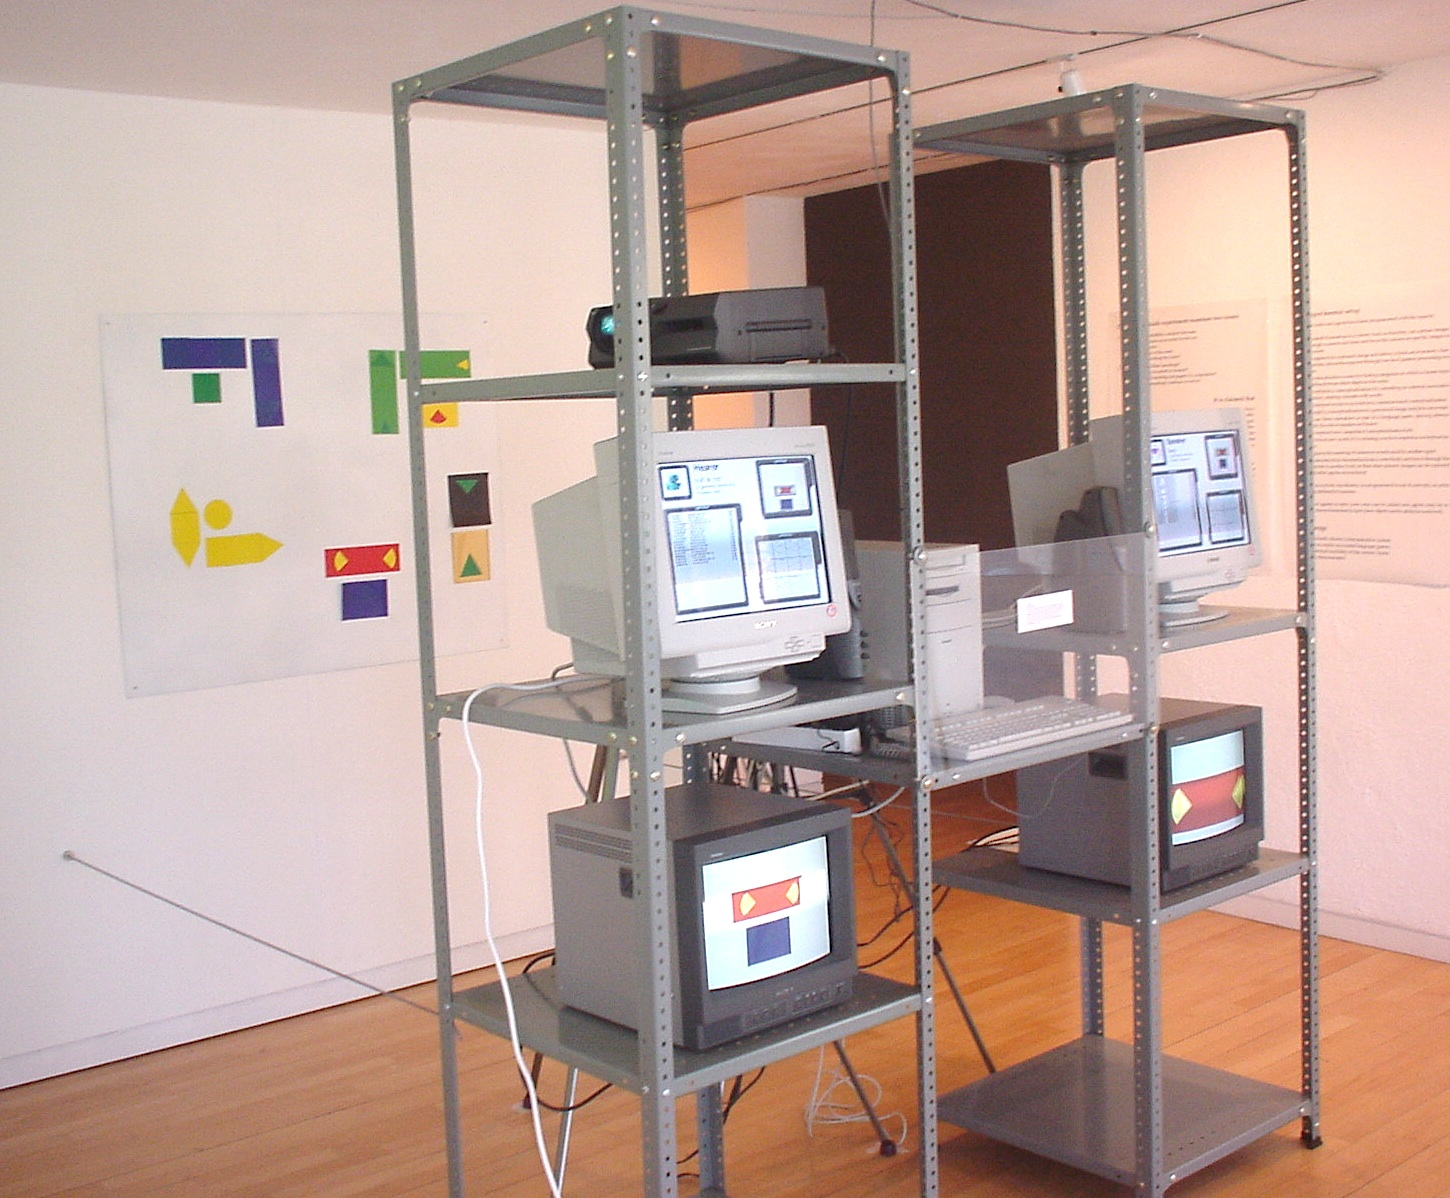
\includegraphics[width=.75\textwidth]{chap9/figs/cambridge-view}}
\caption{\label{fig:sideview} 
View through the street window inside the Kettle's Yard gallery in Cambridge. The cameras are located before 
the towers. The geometric figures are attached to the wall and explanations of the experiment are located on the right.}
\end{figure}

The N01SE exhibition was curated by Adam Lowe (see \figref{fig:lowe}) and Simon Schaffer. 
Adam Lowe is an artist and technologist. He is currently the director of Factum arte (Madrid) which is specialised 
in making life-like replicas of paintings, sculptures and archeological objects, using laser-scanners and 3d printers. 
Recent realisations include the sculptures of Giambattista Piranesi\cite{Lowe:2010}, the 
paintings of Caravaggio and the tomb of Tutankhamun. 
Simon Schaffer is a science historian, professor at the University of Cambridge at the department of History and Philosophy 
of Science. He wrote extensively about the historical developments in scientific research\cite{Schaffer:2011}
and animated television and radio programs, including {\itshape Light Fantastic} (BBC4). 
\begin{figure}[htbp]
  \centerline{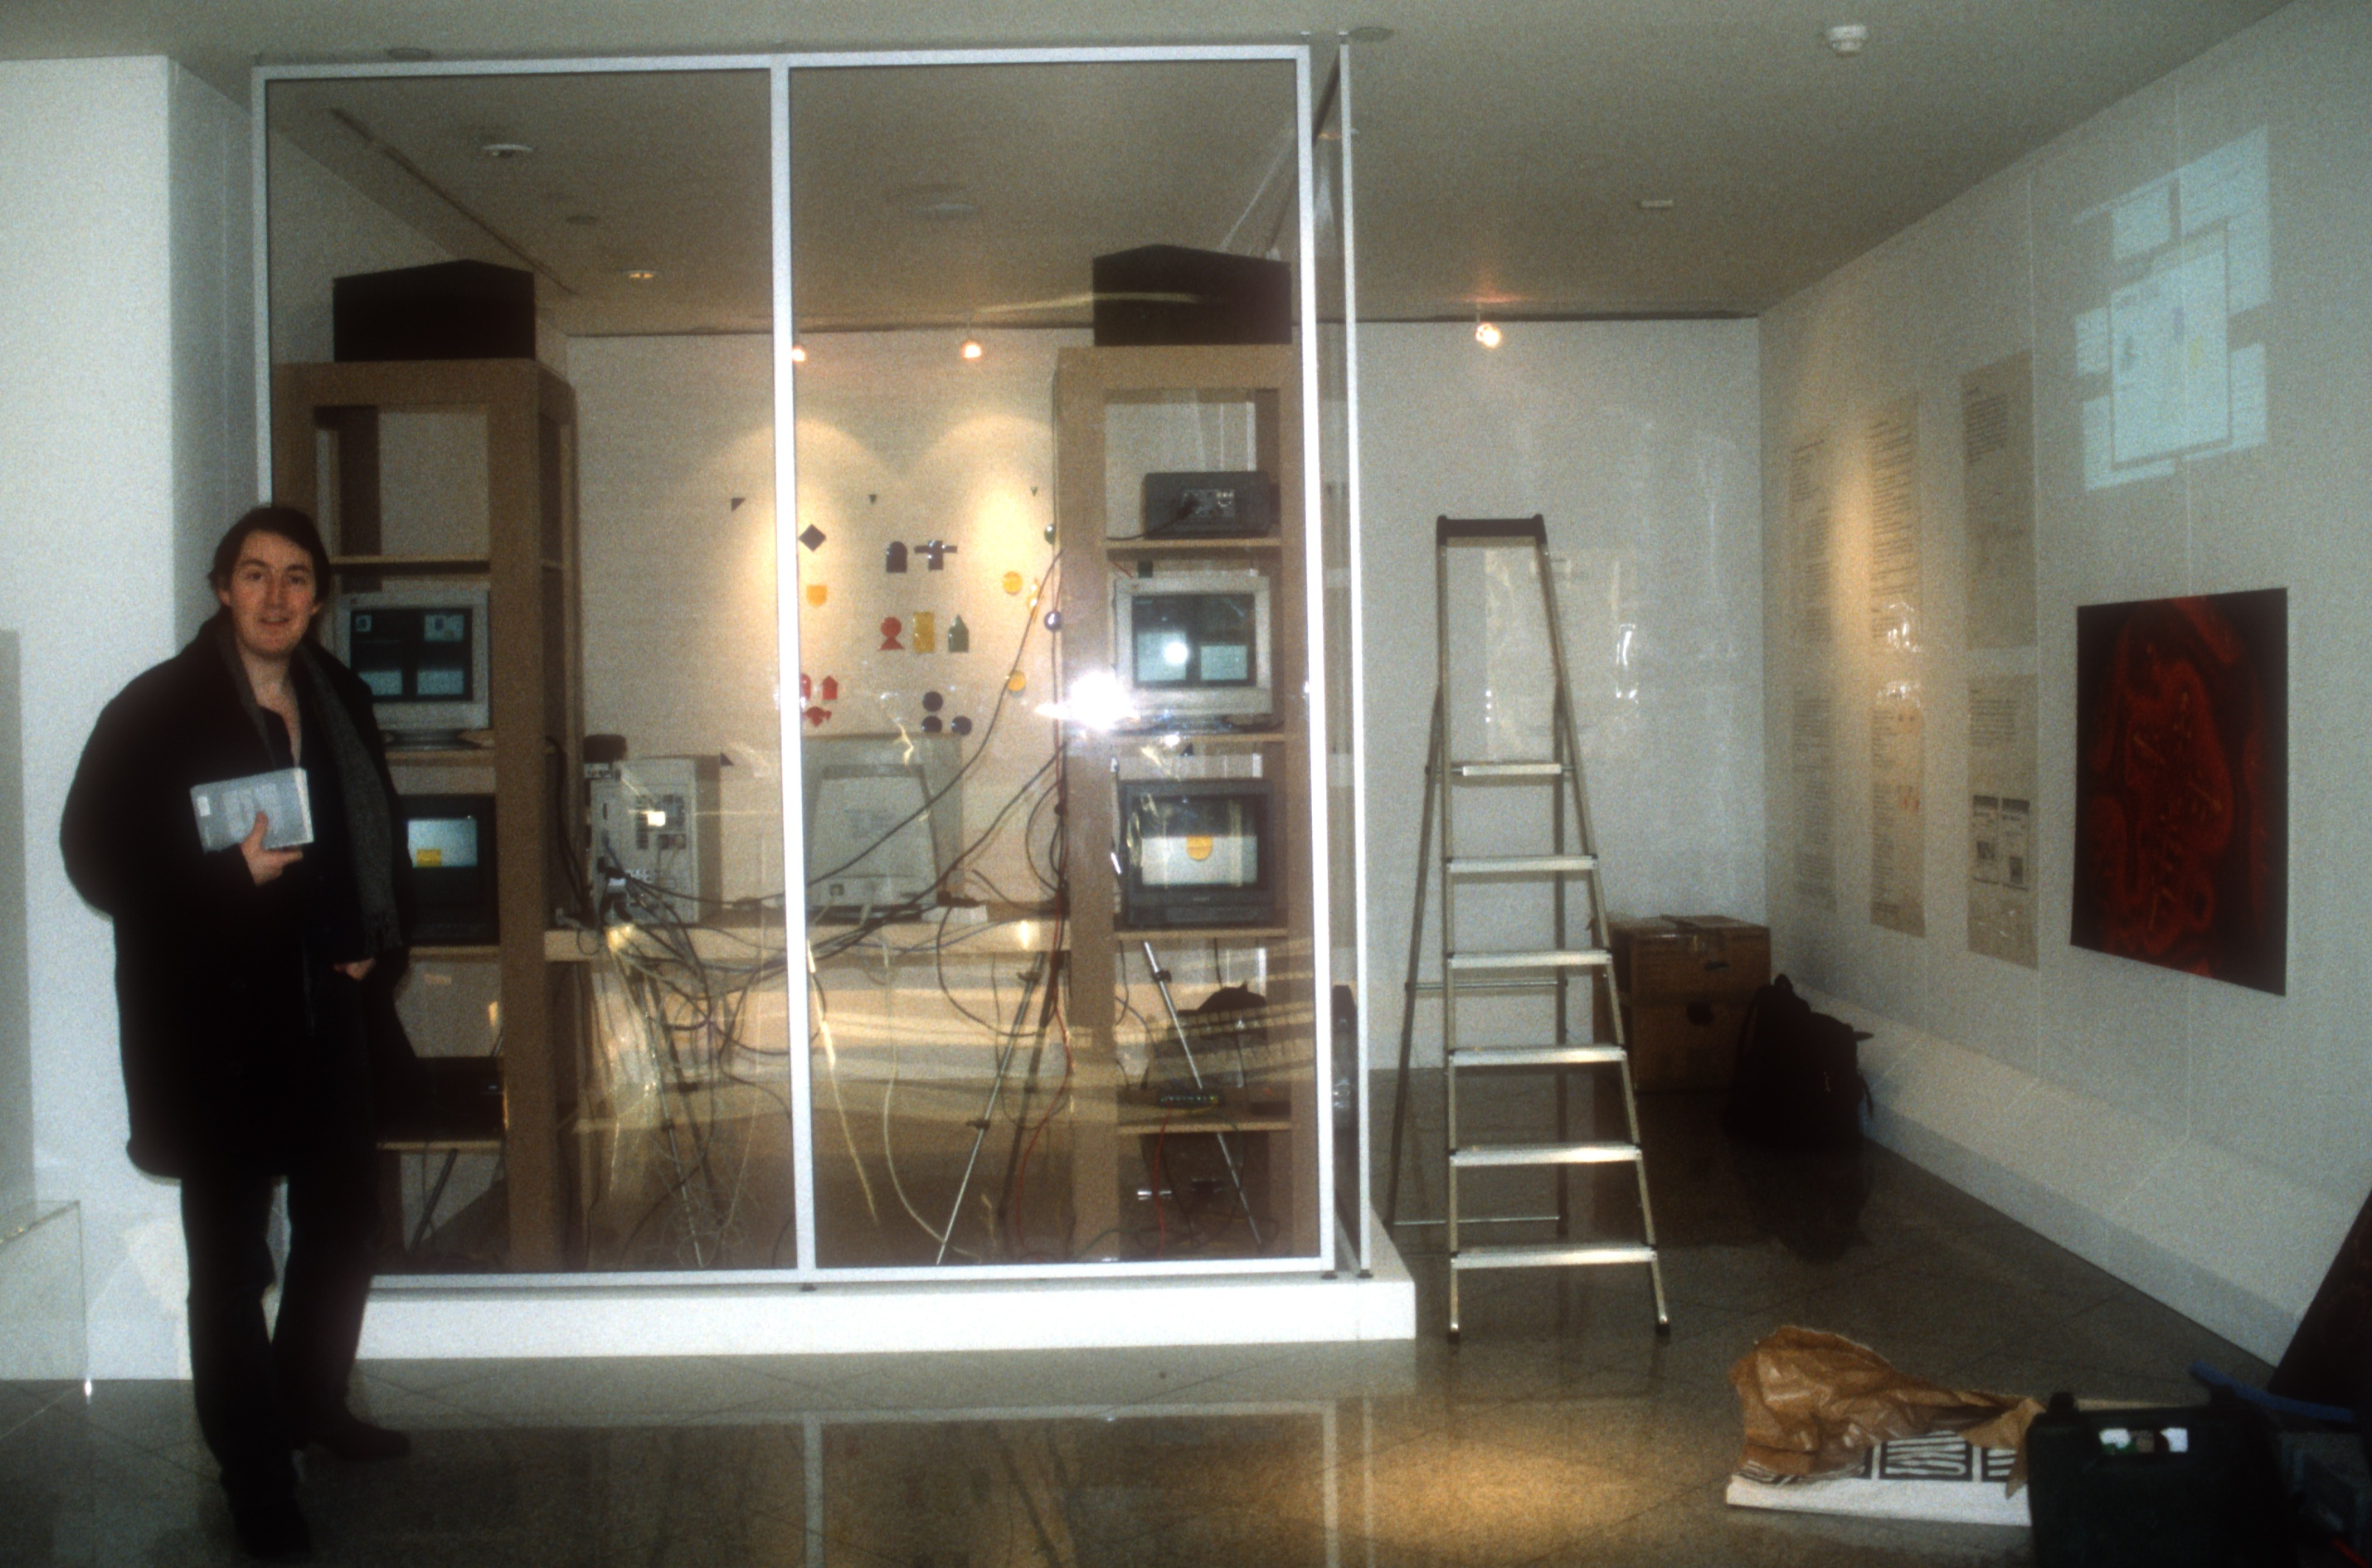
\includegraphics[width=.70\textwidth]{chap9/figs/lowe}}
\caption{\label{fig:lowe} 
Adam Lowe (curator of N01SE) during installation of the Talking Heads experiment at the Wellcome Gallery in London. 
The backwall contained the figures. On the right wall, posters were displayed explaining the experiment.}
\end{figure}

The exhibition was anounced in the following way by its curators: 
\begin{quotation}
{\itshape A multi-site multimedia exhibition in Cambridge with ``realtime" links to London, organised around three key themes in ``digitality":
\begin{verbatim}
   Universal Language 
   Pattern Recognition 
   Data Synaesthetics
\end{verbatim} 
N01SE is not limited to electronic media, but traces the digital imagination from such myths as Noah's Ark, through the early modern experiments of Charles Babbage's Difference Engine and Morse's Telegraph, up to today's charge coupled devices (CCDs), robotics and beyond ...

Displays highlight digitality in history, technology, art and science, drawing upon a wide range of objects and images from artists and scientists around the globe -- everything from 3000BC artefacts to the latest state-of-the-art pictures of the surface of atoms. 

Not a virtual reality "hall of mirrors", but a cultural gallery of hard (and fuzzy) fact.

n01se celebrates the world as signal-and-noise -- the constant simultaneous creation of content with discontents, as communication society filters "meaningful" messages from background "babble" . . . and back again. Ingenuity, serendipity and excess all play up the sensory wonderment of N01SE: The Digital and Its Discontents.

N01SE is news. It's the nuisance others make, a cacophony which prevents us being heard, or even thinking. 
Now the big noise is digital, offering us an escape from disorder by arranging, preserving and transmitting 
information. But is the cloudless noiseless world of digital technology the truth? 

N01SE, hazy images and sudden sparks, random mutations and puzzling glitches, can all become the sources of innovation 
and beauty. 

N01SE celebrates the essential excess from which information is drawn. It probes many different ways of seeing and 
being in the world. Chances are your own sense of order is already someone elses N01SE.}
\end{quotation}
%\begin{figure}[htbp]
%  \centerline{\includegraphics[width=.95\textwidth]{chap9/figs/latour}}
%\caption{\label{latour} 
%Luc Steels Discusses The N01SE exhibition with Bruno Latour who intensively followed the experiments already from the first series at the Laboratorium exhibition in Antwerp. His comments significantly improved the initial designs.}
%\end{figure}

\subsection{Installation at Kettle's Yard in Cambridge} 

The Kettle's Yard Gallery is associated with Cambridge University. It acted as the main site of the N01SE exhibition 
and showed a variety of historical artefacts (including the brain of Babbage and the original DNA structure built by 
Watson and Crick) together with new artistic works. The catalog published by the Kettle's Yard 
Gallery (www.kettlesyard.co.uk/noise) featured articles by Brian Smith, Umberto Eco, Bruno Latour, 
Bruce Sterling, Luc Steels, Peter Weibel and others. Below is the text by Luc Steels as it appeared in the catalog: 
\begin{quotation}
``Meanings are not a priori Platonic entities independent of language; meanings are the result of embodied interactions with the world, obtained via the role words play in verbal interactions called ``language games''. The Talking Heads Experiment explores one kind of language game: a guessing game played by two robotic agents about the scene directly in front of them. One agent acts as Speaker and attempts to draw the attention of the Hearer to some object by transmitting a verbal description of it; the Speaker succeeds if the Hearer correctly guesses which object is ``meant".

To play the game, the Speaker segments the scene and performs pattern recognition to extract features - area, shape, colour, position - about the segments selected. The Speaker then conceptualises the focus element ``topic" as distinct from those of other segments - be it the largest or the furthest to the left or the green one. Next the Speaker verbalises this conceptualisation using descriptive words selected from its lexicon. The Hearer works the other way around; it queries the words transmitted by the Speaker and applies the resultant meanings back to the scene to find what topic the Speaker intended.

To express conceptualisations, agents need a lexicon relating words to meanings. It must function bi-directionally (words-to-meanings and meanings-to-words); it must also store synonyms (more than one word for the same meaning) and ambiguities (more than one meaning for the same word). The agents have not been given a lexicon; they must acquire their own common lexicon as a bi-product of the game.

New words accrue in two ways: either an agent creates its own new words from random combinations of syllables; or it stores transmitted words together with possible-meaning guesses inferred from the scene, then uses a hypothesis-test strategy to render lexicons mutually compatible. Agents keep a running score for every word-meaning pair in their lexicon. When word-topic recognition succeeds the score for that pair goes up, and that of other alternates goes down. This dynamic forces the lexicon of each individual agent toprogressively conform, and keeps it adapting to any language changes or new meanings that need to be expressed. During the course of the exhibition, a group of robotic agents autonomously constructs a shared language about real world scenes in front of them. Humans can interact with the installation through the Internet; they can teach their agents words and follow the general progress towards the construction of the language.

Intriguing questions: How to bridge the enormous gap between the noisy real world of images and behaviors, and the discrete digital world of symbols and language required for communication and thought? How do language and meaning originate? Why do languages keep changing so as to adapt to the needs of their users? How can a language be transmitted between generations without any central coordination nor telepathy?

The installation consists of two computer-controlled robotic camera heads that capture images from `scenes' in front of them consisting of colored geometric shapes pasted on a magnetic whiteboard. The configurations on the board can be changed at any time, making the robots' world unpredictable and open.

Two robotic structures will be active in this exhibition: one at Kettle's Yard in Cambridge and another one at the Wellcome Institute in London. along with additional installations in Brussels, Paris, Tokyo and elsewhere. A website has also been created for the experiment (http://talking-heads.csl.sony.fr/)\footnote{This website is no longer operational but some remnants can be accessed here: 
https://ai.vub.ac.be/talking-heads/} 
allowing anyone to create new agents. People can teach them words, so that elements of human natural languages can sneak into the emerging vocabulary. The agents are autonomous and do not necessarily stick to the words given to them but try to maximally adapt to the behavior of the group and invent their own words. Through the website it is also possible to monitor the progress of the experiment: the lexicon being created, the success rate, the coherence among the agents, the complexity of the language, etc. There is a Hall of Fame listing the best speakers and hearers. This motivates humans to take care of their agents thus ensuring that they move to the top in the Hall of Fame.

The creation of a shared language by a group of autonomous distributed agents is extraordinarily difficult because there are many sources of noise, in the form of disturbances that cause incoherence between the agents:

\begin{itemize} 
\item Two embodied grounded agents always see the situation from different points of view so that they capture different images. Consequently they may have divergent perceptions and hence great difficulty to arrive at a successful game. 
\item The word(s) transmitted may not be accurately produced or received. For example, one agent may produce "wabaku" but the other agent may hear "mabaku". This introduces noise in the signal itself and hence possibly confusion among the agents. 
\item A scene can usually be conceptualised in many different ways, so that there is seldom certainty among the agents whether they share the same meaning. This causes great difficulties in learning the meaning of unknown words. 
\item The lexicons and conceptual repertoires are never exactly the same as each agent develops them autonomously. This generates in additional sources of confusion.
\end{itemize} 
Any theory claiming to explain the origins of word-meaning must confront the handling of noise head on.

Noise plays yet another role, namely as a motor of language evolution. Indeed natural lexicons evolve - even if there are already perfectly good words in a language. Noise on the word form causes changes in the form which propagate in the remainder of the population. Misunderstandings may destabilise a word and cause its meaning to shift.

Another factor in language evolution is due to changes in the environment. Thus two alternative meanings for a word may be compatible for a while but are then disambiguated when a series of scenes arises in which the two meanings are no longer both applicable. For example, all objects may be both green and small and therefore there may be a word "sesubipu" which may mean both, until a clear situation arises where a green object is no longer the smallest and a misunderstanding arises.

Semiotic evolution is continually present. Different meanings for a particular word will emerge over over a large number of language games. During specific periods, different words dominate. The word "droite" (originally introduced by a French speaker) gains the dominant meaning "to the right", then shifts to "at the bottom", and then to "very much to the right". Particularly the words introduced by humans have a tendency to undergo this kind of strong evolution because human users do not know which meanings their agents employ.

How to bridge the enormous gap between the noisy real world of images and behaviors and the discrete, digital world of symbols and language required for communication and thought? How do language and meaning originate? How do languages keep changing yet remain adapted to the needs of their users? How can a language be transmitted between generations without any central coordination nor telepathy?

What is most remarkable about this experiment, is that the robotic agents do not come with pre-programmed ways of conceptualising reality but have to develop their own concepts.

Each agent has been given a mechanism to `grow' new distinctions by expanding discrimination trees. Each tree discretises one sensory dimension. For example, there is a tree for the area of a segment (scale with respect to the image) which divides the range of possible values into two discrete regions, which would be named in English "small" and "large"Other trees focus on position (left versus right or top versus bottom), shape (rectangular or oval), color, etc. Trees can go as deep as necessary to carve out smaller and smaller subregions of a continuous space.

The nodes of the discrimination trees grow in a random fashion but the distinctions that are not successful in the game are pruned. This way the conceptual repertoire of an agent can continue to adapt to the needs of the agent.

How do agents manage to reach coherence in their lexicons without a central coordinator and despite all these sources of noise? The answer is self-organisation. Coherence is reached in the same way as an ant society manages to form a coherent path between a food source and the nest, namely by a positive feedback loop. In this case, there is a positive feedback loop between use and success: The more a word is successful, the more it is chosen by the agents, and the more success it will have. This causes the agents to settle in an attractor where they all prefer the same word for the same meaning and vice-versa. We see a damping of synonymy as in the case of natural languages. Noise has the beneficial impact of getting agents out of attractor states (so called local minima) which are not optimal from the viewpoint of the whole although they are a possible solution.

How do agents manage to share their conceptualisation of the world without their concepts being innately given (pre-programmed) nor centrally coordinated? The answer is structural coupling, another concept adopted from biology. Two systems have a structural coupling if one creates a context for the other and vice-versa, so that each system develops to be maximally co-ordinated without any prior design or global control. The conceptual system and the lexicon of each agent is structurally coupled in the sense that agents prune distinctions that are not successful in the language game, and conversely they keep the ones that are useful and successful. This makes the conceptual system progressively well adapted both to the scenes encountered by the agents and the lexicons used in the group. Sources of noise are again beneficial to foster structural coupling. First of all they help the group to push towards the use of categorisations that are robust against noise. Second, they help agents to explore alternatives and avoid them getting stuck in sub-optimal behavior.

A website has been created for the experiment (http://talking-heads.csl.sony.fr/). Through this site, anybody who wants can create new agents and follow their progress. Owners of agents can teach them words, so that words already used in human natural languages sneak into the emerging vocabulary. The agents are autonomous and do not necessarily stick to the words given to them but try to maximally adapt to the behavior of the group and invent their own words. Through the website it is also possible to monitor the progress of the experiment: the lexicon being created, the success rate, the coherence among the agents, the complexity of the language, etc. There is a Hall of Fame listing the best speakers and hearers. This motivates humans to take care of their agents thus ensuring that they move to the top in the Hall of Fame.

To express a conceptualisation, agents need a lexicon relating words with meanings. The lexicon must be consultable in both directions (from words to meanings and from meanings to words). It must be able to store synonyms (more than one word for the same meaning) and ambiguities The agents have not been given a lexicon a priori. They have to acquire their own lexicon as a side effect of the game. New words get into a lexicon in two ways: When an agent has no word to express a particular distinction, the agent can create a new one by a random combination of syllables. When an agent hears a word that he does not know, he stores the new word with his own guess of what the meaning could be in the scene being perceived.

Agents then use a hypothesise-and-test strategy to make their lexicon compatible with the rest of the group. They keep a score for every word-meaning pair in their lexicon. When a word has success in the game, the score goes up, and its competitors go down. When the game fails, the score of the used word(s) goes down. This creates an inhibition-excitation dynamics making the lexicon of the individual agent progressively conform to the most successful lexicon of the group. It also ensures that an agent's lexicon keeps adapting if the language changes or if new meanings need to be expressed."
\end{quotation}

\subsection{Installation at the Wellcome Gallery in London} 

The second installation during the N01SE exhibition was installed in the Wellcome Gallery in London 
(see \figref{fig:program}) 
from 22 January until 26 March 2000. This gallery is associate with the Wellcome trust and featured additional 
art works by Joseph Grigley, Evgen Bavcar, Manuel Franquelo, Garret and Jones, and Giles Revell. The local curator
Denna Jones described the exhibition as follows: 
\begin{quotation}
{\itshape Digitality is transforming traditional ways of thinking about the impact of technology on culture. This exhibition 
looks at how complex structures can be transformed, translated and transmitted changing the nature of communication. 
A multimedia multi-site exhibition, N01SE demonstrates how language and our five senses can be changed or 
enhanced through 'digitality, and introduces visitors to pioneering developments in cross-disciplinary art and 
science.}
\end{quotation}
\begin{figure}[htbp]
  \centerline{\includegraphics[width=.60\textwidth]{chap9/figs/NOISE-programmaboek}}
\caption{\label{fig:program} 
Catalog cover and poster of the N01SE exhibition at the Wellcome Gallery in London.}
\end{figure}

The installation itself was similar to the one in Cambridge. There was a wall with 
geometric figures pasted on it, posters explaining the exhibition, the two pan-tilt cameras mounted on tripods, 
and the computers driving the software (see \figref{fig:london-heads}). The London site posed particularly hard 
problems in the alignment of the cameras. 
It turned out that a subway was passing under the gallery and causing strong vibrations 
every few minutes, which caused the cameras to physically shift on the floor. Because the pointing behavior was sensitive 
to alignment and prior calibration, this lead to growing pointing errors and 
subsequent errors in feedback, causing a strong decline in 
the success rate and occasional chaos in the agents' vocabularies. This was partially offset by stable conditions in 
other sites but nevertheless made the task of reaching coherence virtually impossible. 
\begin{figure}[htbp]
  \centerline{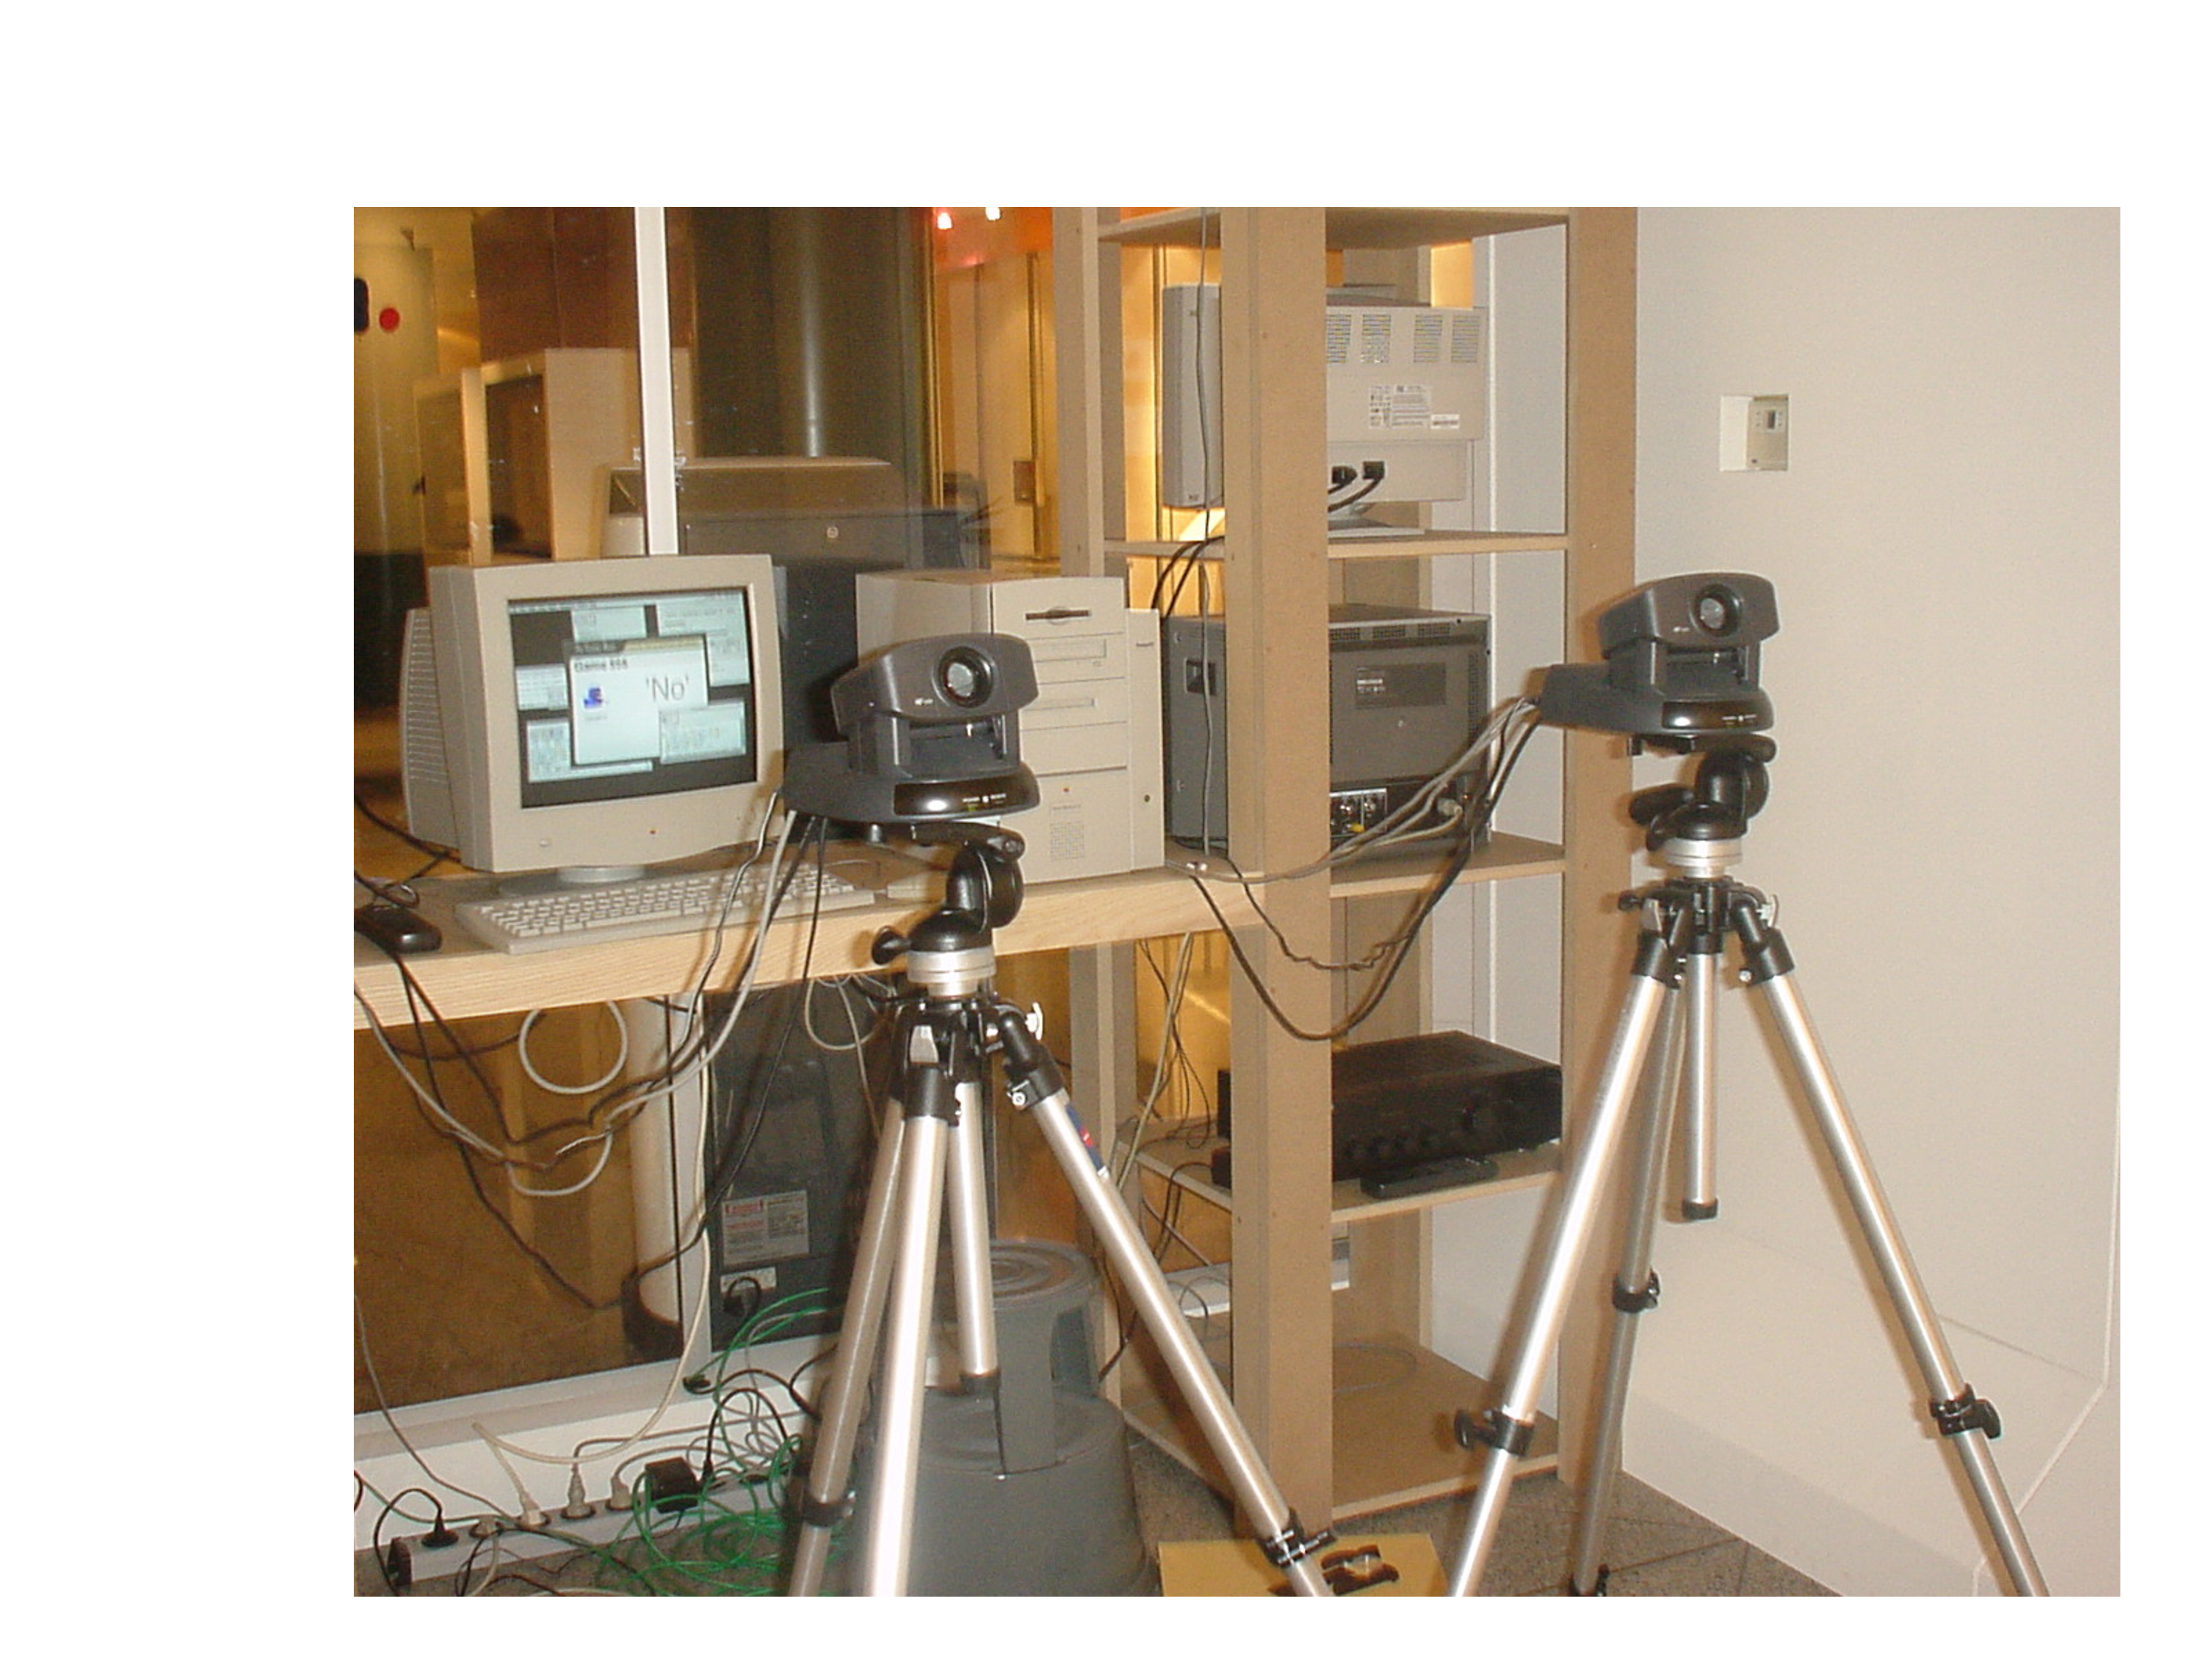
\includegraphics[width=.55\textwidth]{chap9/figs/london-heads} 
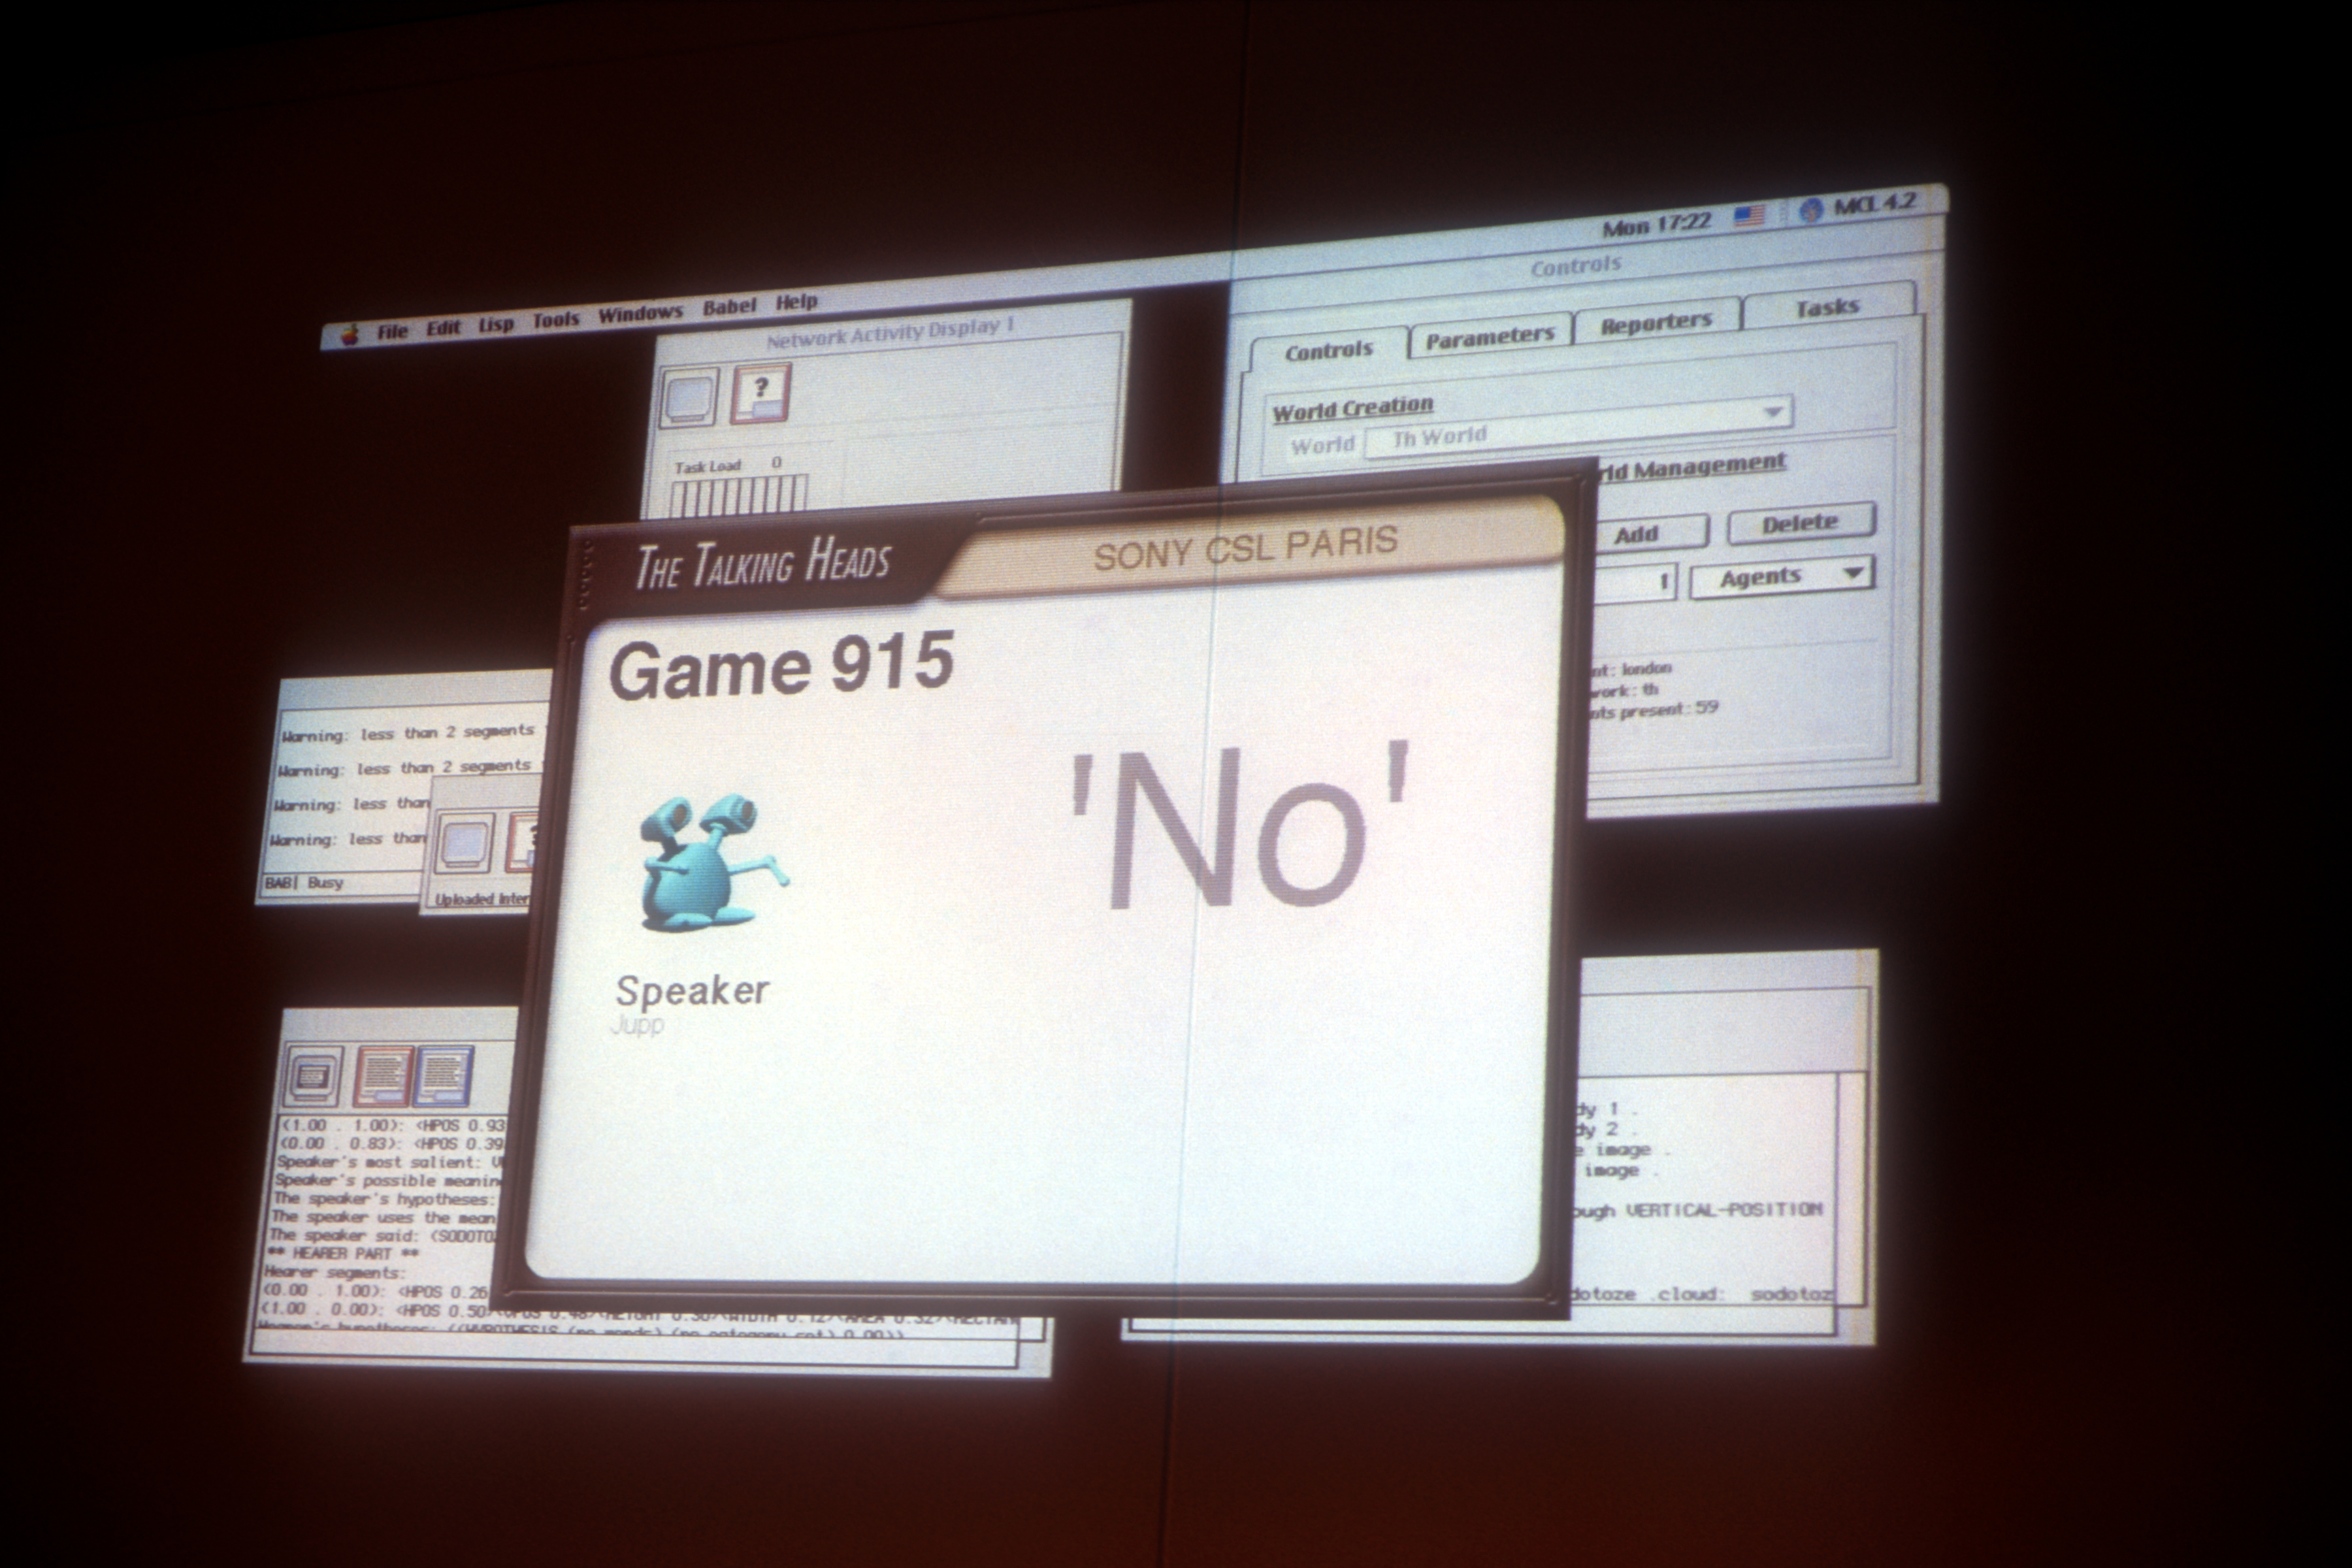
\includegraphics[width=.44\textwidth]{chap9/figs/screen}}
\caption{\label{fig:london-heads} 
Installation at the Wellcome Gallery in London. Left. Talking Heads cameras oriented towards the wall on which 
geometric figures were pasted. Right. Projection of interaction during ongoing experiment. A game just failed and 
the speaker says "no".} 
\end{figure}

The exhibition catalog, assembled by Denna Jones, contained the following text by Luc Steels: 
\begin{quotation}
``The Talking Heads Experiment is a collective effort of members of the Sony Computer Science Laboratory, Paris
and VUB Artificial Intelligence Laboratory Brussels, in particular Luc Steels, Fr\'{e}d\'{e}ric Kaplan, Angus McIntyre, 
and Johan Van Looveren. This research has been sponsored by the Sony Computer Science Laboratory in Paris and a 
GOA grant from the Belgian government to the VUB AI Lab. 
\begin{enumerate}
\item How can a cognitive agent bridge the enormous gap between the noisy real world of images and behaviours and 
the discrete, digital world of symbols and language required for communication and thought? 
\item How do language and meaning originate? How come languages keep changing and how do they remain adapted to 
the needs of their users? How can a language be transmitted between generations without any central coordination 
nor telepathy?
\end{enumerate}

\noindent
{\bfshape Situated robots and teleports}

\noindent
The installation consists of two robotic heads. These are steerable cameras controlled by a computer that hosts the 
architecture and knowledge state of each agent. The robots capture images from scenes in front of them. The scenes consist 
of coloured geometrical shapes pasted on a magnetic white board. The configuration on the board can be changed at any 
time, making the robots' world unpredictable and open. The robot infrastructure is connected to the Internet, so 
that an agent may dematerialize from a body and travel over the internet to another body in which it can re-materialize.
Two robotic structures will be active as part of the N01SE exhibition: one at Kettles'Yard in Cambridge and another 
one at the Wellcome Trust Two10 Gallery in London. 

There will be additional installations in Brussels, Paris, Tokyo and other places. The agent teleporting facility 
makes it possible to have thousands of robotic agents and to confront each agent with many different scenes. 

\noindent
{\bfshape Constructing perceptually grounded concepts}

\noindent
What is most remarkable about this experiment is that the robotic agents do not come with 
pre-programmed ways of conceptualizing reality but have to develop their own concepts. Each agent has been 
given a mechanism to 'grow' new distinctions by expanding discrimination trees. Each tree discretizes one sensory 
dimension. For example, there is a tree for the area of a segment which divides the range of possible values
into two discrete regions, which would be named in English 'small' and 'large'. Other trees focus on position 
(left versus right or top versus bottom), shape (rectangular or oval), colour, etc. 

Trees can go as deep as necessary to carve out smaller and smaller subregions of a continuous space. The nodes
of the discrimination trees grow in a random fashion but the distinctions that are no successful in the game are 
pruned. This way the conceptual repertoire of an agent can continue to adapt to the needs of the agent. 

\noindent
{\bfshape Sources of noise}

The creation of a shared language by a group of autonomous distributed agents is extraordinarily difficult 
because there are many sources of noise, in the form of disturbances that cause incoherence between the agents: 
\begin{itemize} 
\item Two embodied grounded agents always see the situation from different points of view so that they capture 
different images. Consequently they may have divergent perceptions and hence great difficulty to arrive at a 
successful game. 
\item The word(s) transmitted may not be accurately produced or received. For example, one agent may produce 
'wabaku' but the other agent may hear 'mabakau'. This introduces noise in the signal itself and hence 
possibly confusion among the agents. 
\item A scene can usually be conceptualized in many different ways, so that there is seldom certainty among 
the agents whether they share the same meaning. This causes great difficulties in learning 
the meaning of unknown words. 
\item The lexicons and conceptual repertoires are never exactly the same due to the fact that each agent
develops them autonomously. This brings in additional sources of confusion. 
\end{itemize}
Any theory claiming to explain the origins of word meaning must confront the handling of 
noise head on. 

\noindent
{\bfshape Cultural evolution}

\noindent
Noise plays yet another role, namely as a motor of language evolution. Indeed natural lexicons evolve - 
even if there are already perfectly good words in a language. Noise on the word form causes changes 
in the form which propagate in the remainder of the population. Misunderstandings may destabilize a
word and cause its meaning to shift. 

Another factor in language evolution relates to changes in the environment. Thus two alternative 
meanings for a word may be compatible for a while but are then disambiguated when a series of scenes
arises in which the two meanings are no longer both applicable. For example, all objects may be both 
green and small and therefore there may be a word 'sesubipu' which may mean both, until a clear 
situation arises where a green object is no longer the smallest and a misunderstanding arises. 
\end{quotation}

\section{Iconoclasm} 

The second series of Talking Heads experiments which were part of the N01SE exhibition,
featured again a website with which human users could create their own 
agents, teach them words by going through images of past games, and send them off on the teleportation network.\is{iconoclasm}
In the first series, a
large group of users participated, posting enthusiastic commentaries on the forum, suggesting improvements 
to the interface, and discussing possible theories of language evolution. Unfortunately, during the second 
series, a group of students mostly from the university of Hull (UK) evolved from enthusiastic and interested 
participants into a mob of rude thugs that wanted to destroy the experiment at all cost, stimulated by 
local curator Denna Jones and insiders at the Wellcome Gallery, who apparently were strongly opposed 
that the N01SE exhibition took place 
at their location and somehow had a personal crutch against Adam Lowe, global curator of the N01SE initiative. 
This iconoclastic event was (in the year 2000) a forerunner of the damage that 
hackers have been inflicting on the web, destroying the spirit of collaboration and 
sharing with which the web was founded. 

The British hackers realised that they could give 'dirty' names to their agents and, because they 
could teach their own agents these words, they could also teach their agents 'dirty' words for colors, 
shapes, or any other concept that agents were using. These words would unavoidably propagate in the population. 
As these hackers were extremely active, creating many agents, continuously launching them to different sites, and teaching 
their agents words, the global vocabulary progressively became unacceptable. 
The installations were in public spaces visited by school children, and so concern grew with the exhibition organisers
at other locations (except the London site where those responsable actively encouraged this destructive behavior). 
As a response, the experiment was temporarily halted and provisions put in to avoid that a small group would have 
excessive influence. It was still possible to provide a name to your agent and teach your agents words but 
some form of decency had to be respected. This change restored order but resulted in an overreaction of the part of 
the English hacker group who now used all possible means to attack the Talking Heads servers themselves, 
enouraged by Denna Jones and aided by others at the Wellcome Gallery. 

This episode showed a phenomenon that a decade later has become very common. The web is far from an idealistic common 
ground through which people can exchange ideas and tools. It brings out the worst in some people, particularly 
if there is a mob effect in which different individuals with unstable ethical values 
push each other to do things they would otherwise not do. 

It is instructive and rather fascinating, particularly from a sociological and anthropological point of 
view, to follow the dialog on the Talking Heads Website Forum between the main protagonists of the story.
It went from enthusiastic interaction and experimentation to aggressive and hateful 
destruction. The misspellings, grammatical errors and foul language they produced have been left into the text. 
Only a small fraction of the dialog is reproduced here.  

We pick up the dialog on the 25 of february 2000. Until that date the forum was very active both 
with general discussions about the future of intelligence or the origins of language, and with specific questions, mostly 
why agents were so slow in playing games. Many users were too impatient and did not seem to realise that playing 
a language game could easily take a minute or two. However the major problem was the deviating alignment of the cameras, 
which had to guarantee that there was a common frame of reference between the agents, and hence the 
possibility of sharing attention. The cameras were mounted on tripods. When somebody accidentally 
moved the tripod, the frame of reference was no longer exact. As mentioned earlier, traffic (particularly subway 
traffic in London) caused vibrations of the cameras so that they kept shifting and getting out of balance. 

A group of University of Hull students (with names like Trash, yeah8a8y, schedski) 
became very much involved. They 
communicated through the Forum using often slang and sexist language and making a surprising 
number of spelling errors and grammatical mistakes. The group had been 
trying to impose their own language by very actively teaching their agents and sending them to the same site, namely 
Paris, which they had noticed had the most stable operating conditions. This worked (as indeed it was supposed to) 
at which point they decided to do the same with the London site although the camera 
alignment was too unreliable to allow the evolution of a stable language. 

{\small
\rule{0.8\textwidth}{.4pt}\\
{\bfshape 2000-02-25 21:37:24 Yeah8a8y}\\
{\itshape Paris}\\
"Hey there peeps... Thanks to the greatness of yeah8a8y, Paris has a great success ratio... Oh yeah with a little help from TRASH.... Ok a lot of help... Heres to Paris!!!\\
The next server to be conquered is London!!!"\\
\rule{0.8\textwidth}{.4pt}\\
{\bfshape 2000-02-25 21:40:13 Yeah8a8y}\\
{\itshape RE: Paris}\\
And you may notice the succes of a few of our words on the Lexicon.... God the greatness of a couple of wasters from Hull Uni, three days to conquer a server... Didn't think much to those Frenchies anyway!!!!!\\
\rule{0.8\textwidth}{.4pt}\\
{\bfshape 2000-02-25 21:52:23 Trash}\\
{\itshape RE: Paris}\\
"Yeah London being the capital of the greatest country in the world and currently last in the server league well if we can get them frogs to say words the brits WILL CONQUER\\
\rule{0.8\textwidth}{.4pt}\\
{\bfshape 2000-02-25 21:55:49 Trash}\\
{\itshape YELLOW MK 1 ESCORT}\\
Hey mate nice seeing you around paris !!!! Enjoy the company especially since you know most of our words AND get the Biatches right... you can have my sister anyday... so then mate see ya round keep driving the crap car.	
Have noticed the absence of fine ass girls in here am i wrong.... hope soooo.\\
}
\rule{0.8\textwidth}{.4pt}\\

At this point, they realised that the London alignment was off and this is the first time that Phlox (as Denna 
Jones called herself) intervened. She immediately shows
a negative attitude towards the experiment triggered by her personal conflict with Adam Lowe. 
Colleagues of hers (fish and A Londoner) respond with inside joke
remarks that the Hull group does not understand. Fish had been trusted with admin passwords because he
was responsable for maintaining the London site, but he greatly abused this trust as the experiment proceeded. 

{\small
\rule{0.8\textwidth}{.4pt}\\
{\bfshape 2000-02-25 22:02:36 LondonCalling}\\
{\itshape CALIBRATION OF CAMERAS London}\\
"Can London PLEASE calibrate their cameras???? PLEASE!!!!!\\
\rule{0.8\textwidth}{.4pt}\\
{\bfshape 2000-02-26 16:52:32 Yeah8a8y}\\
{\itshape RE: CALIBRATION OF CAMERAS London}\\
very good.... Absolutely no chance of Domination if the cameras arn't calibrated... SORT IT!!\\
\rule{0.8\textwidth}{.4pt}\\
{\bfshape 2000-03-02 15:46:50} phlox\\
{\itshape RE: CALIBRATION OF CAMERAS}\\
i manage the two10 gallery in which the talking heads display is currently installed. would that it were so simple to sort it and keep the cameras correctly calibrated. all equipment was installed by the brussels group and whenever the cameras need calibrating - for whatever reason - it means one of the brussels boffins has to pop over to fix it. they've been over once since the exhibition opened and decided to move the cameras forward 2 feet. not really an exact science is it? the grand master - luc steels - is coming to the gallery tomorrow, so perhaps he will enlighten me as to why the cameras seem to need constant calibration, and i'll let you know. cheers.\\
\rule{0.8\textwidth}{.4pt}\\
{\bfshape 2000-03-02 20:04:52 fish}\\
{\itshape RE: CALIBRATION OF CAMERAS London}\\
that's as maybe, phlox, but i'm guessing you secretly come into the exhibition and kick the cameras when 
you're in a bad mood, like say when someone has been horrid to you.\\
\rule{0.8\textwidth}{.4pt}\\
{\bfshape 2000-03-03 20:08:36 schedski}\\
{\itshape RE: CALIBRATION OF CAMERAS London}\\
wassup fish?\\
\rule{0.8\textwidth}{.4pt}\\
{\bfshape 2000-03-03 23:06:43 fish}\\
{\itshape RE: CALIBRATION OF CAMERAS London}\\
come on, admit it, you guys there spend all day stomping around your exhibits, breaking the displays, unplugging the monitors and generally mucking things up. i'm surprised london's still got two cameras even working and they haven't already been flogged down some boozer for a monkey and a couple of jellied eels\\
\rule{0.8\textwidth}{.4pt}\\
{\bfshape 2000-03-07 13:03:46 A Londoner}\\
{\itshape RE: CALIBRATION OF CAMERAS London}\\
Well, if you people will confuse the poor things with your outrageous diction, they might know which way to point... One of them was practically in tears the other day as I watched it shaking its head in disbelief at the language it was meant to repeat. What ever happened to 'Adam's a cool bloke'?\\
}

Meanwhile the Hull group is pursuing and explaining their particular experiment that they carry out within the 
Talking Heads framework. The experiment itself is interesting and shows that they understand what is 
going on and are creative. Also the overall dynamics is working. The group realises that a language can form 
on its own or that it can be influenced by humans teaching agents their own language. 
At the same time, there is already one user (called Cheesy) who is pushing to introduce
dirty words to the agents. He does not belong to the Hull group but is most probably somebody from the 
Wellcome Gallery already trying to put the N01SE exhibition in a bad light. \\
{\small
\rule{0.8\textwidth}{.4pt}\\
{\bfshape 2000-02-25 22:55:28 Norton}\\
{\itshape Teaching}\\
While participating in this experiment seemed quite interesting - I'm simply not getting it. When I try to comprehend what is meant by certain words so that I can teach my agents - I cannot understand the distinctions made.  Does anyone get it? \\
\rule{0.8\textwidth}{.4pt}\\
{\bfshape 2000-02-26 16:47:55 Yeah8a8y}\\
{\itshape RE: teaching}\\
The best thing to do is to leave them for a number of games... Like the tips say 'bout 50... then start looking at the words they use, have to be successful tho'... then teach your other bots this word for that picture! It is a bit hit and miss tho' coz a lot of words are ambigious (?Sp) and mean different things... remeber it is actual properties and not usually shapes... But you can have success! Check out some of mine and Trash's word in the top 20 lexicon, Hullcitynutter,eightyfiftyone, msixtytwo, wotsit, mamorys (Childish I know, but hey I'm a student) and you'll realise you can actually do it... Helps if your at Paris tho'!\\
\rule{0.8\textwidth}{.4pt}\\
{\bfshape 2000-02-26 20:41:20 Trash}\\
{\itshape RE: teaching / TRIBES}	\\
Basically think about it like this... On the Earth there are many different languages spoken by people usually in a specific geographical location. Now myself and yeahbaby looked at this experiment (as we are very interested in AI and have done much work in this field) and decided to test the idea of "Tribes" where all those in that tribe speak the same lingo. We also figured that tribes rarely move out of their "Birth Location" so kept them at one site. As can be seen now ALL our Agents speak the same language and have even taught it to others outside the Tribe (such as the esteemed Yellow Mk 1 Escort  and possibly even Anne's little Agent). 
These agents we considert to be forreigners!! But stilll they can communicate with our Agents... If you have noticed our words in the lexicon as explained by yeahbaby have  very few deviations from what was intended unlike others such as "Gumble" which appears to mean Everything!!!!!

This I do beleave Validates mine and my colleagues (Yeahbaby) opinion that language can only evolve in the pressence of small but tightknit communities.

As the next stage we wish to see what happens when 2 "Tribes" get together Hopefully they become multilingual !!.
My theory is thatconfusion of words will be short lived and all will be ironed out after only a few games . Especially if the "tribes" are allowed to consolidate they meanings by once again returning to their own community with little outside  influence....

I am sure you will all agree that personel experiments like these improve this and we would be interested to hear any opinion from others ...... are we doing the right thing or just playing gods etc???
 Does this prove evolution as a basis or is there a need for gods etc.... 

Also anyone interested in settingg up a tribe PLEASE talk to us first as we have much experiance in these matters!\\
\rule{0.8\textwidth}{.4pt}\\
{\bfshape 2000-02-27 14:39:10 Oisin}\\
{\itshape RE: teaching / TRIBES}\\
Perhaps tribes could be created by sending agents to a specific server only eg only paris or only brussels and to see what words develop at the separate servers then switch after 2,4,6 months maybe any suggestions?\\
\rule{0.8\textwidth}{.4pt}\\
{\bfshape 2000-02-27 19:39:10 Trash}\\
{\itshape RE: teaching / TRIBES}\\
You mean by not playing god ???? and letting them get on with it at one site?? .... well yes but the server would have to be locked down by that tribe otherwise you would get outside inflences teaching them stupid like gumble which meanbs everything... it would probably take just 100-300 games each agent to develop a usable language (Aslong as the server has no agents from outside the  tribe in there)\\
By teaching them myslef and Yeahbaby got usable language going in  less than 2 days!!!!!!! Just see the success of most of our words in the lexicon top 20!!\\
God us 2 are good!!\\
\rule{0.8\textwidth}{.4pt}\\
{\bfshape 2000-02-27 19:39:55 smartypants}\\
{\itshape RE: Collusion Tribes}\\
I think the theories that are starting to surface is the most interesting part of the experiment for me. 
I started ignoring the 'teaching' mails as they seemed concerned with the technical side but thanks Trash for pointing out you had posted up your theory (p.s. when you talk about definitions of your words where are these, or are you just talking about studying the images?).\\
The bit that I would like more explanation of ('cause Smartypants is an ironic name) is the bit about the two tribes coming together, especially as Paris is really the only viable option at the moment. I noticed that Virtuoso (the only one of my robots that managed to get into Paris in the last day) was unranked yesterday, but today has jumped to 140ish as both as speaker and a hearer - I guess this is because that one 'tribe' have been forced to cement that language.\\
The trouble is, without a good interpreter (us I suppose), won't it just cause confusion in our robots when they go and meet the other 'dumber' ones? i.e. they teach the others our words, but the others teach them the wrong words back as well.
This means you would keep playing several iterations of the games.\\
My thoughts on collusion were centered around this - we could reduce the iterations by all agreeing on common words to teach our robots, thus perpetrating more of the 'right' words whilst eliminating the 'wrong' words...\\
... any thoughts on my incoherent ramblings??\\
\rule{0.8\textwidth}{.4pt}\\
{\bfshape 2000-02-27 19:52:20	Trash}\\
{\itshape RE: Collusion Tribes}\\
At the minute me and Yeah are off the Paris server (we are regrouping our thoughts for further action!!!)
But yes I did mean view the pictures when i said definition.\\
By 2 tribes I mean obviously two who have been taught on the same server.
So say that i train my agents on there this week and you train your tribe next week on the same server with different words..... when both tribes are capable of good communication we then take half of each tribe and place them together in the 3rd week on the Paris server and see if they become multi lingual.\\
We then sned these linguists back to their own tribe and see what happens.\\
Unfortunately many people have tried to jump on the band wagon of Paris success and send their Agents there with no idea what they are doing ... this has meant that we can not get our tribe to dominate as we would like.....\\
The problems with organising tribe transfer is immense and it is a shame people don't exp[lain what they are doing on this fprum so that all could help out by say teaching their agents the words being used or even evacuating a site so that two tribes can collide ...\\
It is a real shame that an experiment into AI and Language is hampered because people are unwilling to communicate with each other .... \\
Well I guess that those of us who want a proper experiment should just ry their best in difficult circumstances...\\
About the wrong words being taught !!! If your Tribe is more than 60\% of the server then your tribe generallly succeeds in teaching the "foreigners" with little effect on themselves ... This has more to do with Probability than anything else.
\rule{0.8\textwidth}{.4pt}\\
{\bfshape 2000-02-27 20:46:29 smartypants}\\
{\itshape RE: Collusion Tribes}\\
Thanks Trash. I was thinking in different terms...\\
... seeing as anyone doing anything is on the Paris server, I was imagining that as one 'big' tribe and that any outsiders (stuck on the other servers, or new) are the 'other' tribes so thanks for clearing that up for me.\\
I'd be interested in working with you and Yeahbaby for a more meaningful experiment, particularly as loads of 'dumber' robots (by that I mean ones not enjoying the Paris success) will soon be unleashed on us.\\
Just to clarify, my plan up until now was to let my robots learn 40-50 words (as suggested in the tips), I started to teach them the most successful words from the lexicon yesterday (most of which were yours - grrrrrr, jealous!) and then I sent them to Paris. (This was before I started putting stuff up on the forum and saw your theory unfortunately). \\
The only one that got in was Virtuoso, and even then he didn't really get to play enough games as I was experimenting to see if the number of games you choose has any effect on getting into that server.\\
Anwyay, let me know if you're interested (I've only created 7 at the moment).\\
By the way, do I remember seeing somewhere that you're both girls?????\\
... 'cause I am...\\
If so it is interesting to see different ways people approach the experiment. If I was running the experiment I reckon I could do research from the forum, as well as the actual experiment.\\
\rule{0.8\textwidth}{.4pt}\\
{\bfshape 2000-02-28 14:25:01 Yeah8a8y}\\
{\itshape RE: Collusion Tribes}\\
At the moment it seems I can't get on the Paris server for love nor money... Never mind... Anyway Trash has good theories!!! Two particully good tribes at the minute, which also 'collided' ( Wait a minute, Frankie goes to Hollywood anyone? ) on the Paris server are run by me and Trash. There are some other out there (Cheesy) that are more content teaching obscene word to their bots. Anyway by both me and him filling up Paris (Max. of 16 agents from 20 at one point) a successful dialect has been taught between them. We now rank 5 words in top 10, and 9 overall in top 20.  Again Trashs theories ring true. \\
And the bit about words getting taught wrong is more a case of... well if a french person tuaght you the word for "Tower" and you where listening  to someone who understood french, "Tower" would be used in the french wording, but you also retain your interpretation of "Tower" and use this one which you consider more successful in the speaking sense. This is what happened with our own "hullcitynutter" and "lafizana". My agents now understand both, but only seem to say "hullcitynutter"  (Thier original word, not the learnt one)\\
This, of course, all goes out the window  when you yourself teachs them... Maybe another bad aspect of this AI programming.\\
\rule{0.8\textwidth}{.4pt}\\
{\bfshape 2000-02-28 16:24:47 Yeah8a8y}\\
{\itshape RE: Collusion  Tribes}\\
OK no... I'm no girl!!! But there you go... I'm a bloke\\
\rule{0.8\textwidth}{.4pt}\\
{\bfshape 2000-02-28 17:04:23 Yeah8a8y}\\
{\itshape RE: Collusion  Tribes}\\
I'm posed with another problem... As you know Brussels and Paris have been inactive for a bit... do I keep with the project and just send the bots out to Paris... or use this as a change point and educate them in Brussel's...\\
I'm going to stay with Paris... Teach other people the use of the words carefully set out by me and Trash... and generally gather more success!\\
I now have 18 bots by the way most are ranked within the top 100.. 1 or 2 exeptions... anyway I have been successful by sending the all to Paris... for top gamage action \\
It usaully takes all night but there you go... even the Earth took an entire week to sculpture.\\
\rule{0.8\textwidth}{.4pt}\\}
%__________
\noindent
To deal with the problem of agent congestion, software issues, and camera misalignment at the London 
and Cambridge sites, maintenance was carried out which lead to a temporary unavailability of the experiment. 
Surprisingly, the reaction of the Hull group was entirely negative as they saw it as a 
way to prevent them from gaining or keeping control of the language used by the agents, even though 
Angus McIntyre clearly and patiently explained why maintenance was necessary. Also, Denna Jones (Phlox) took 
it personally as she did not realise that the calibration errors were due to vibrations caused by
traffic near and under the Wellcome Gallery.  \\
{\small 
\rule{0.8\textwidth}{.4pt}\\
{\bfshape 2000-03-01 15:28:10 Angus McIntyre}\\
{\itshape Performance, problems and fixes}\\
As some of you have noticed, there've been some problems with this round of the Talking Heads experiment. For one thing, success rates have generally been very low, because the language has never properly stabilised. For another, a large backlog of agents has built up, and there have been considerable delays in getting certain agents to and from servers.\\
We are aware of these problems, and are actively working on fixing them. Part of the problem is that the Talking Heads has been a victim of its own success - lots of people participating enthusiastically makes for lots of agents, with new ones being added every day. Moreover, the Talking Heads is a 'real world' experiment, with real physical moving parts (the cameras) which means that each game takes a certain and non-trivial amount of time. These are just two reasons why things may sometimes move slowly in the world of the Talking Heads.\\
Problems have also been caused by the cameras losing calibration (that evil 'real world' strikes again), so that our agents sometimes seem to be looking at entirely different parts of the scene, something which is bound to cause problems. Last but not least, there turn out to have been some bugs in our software, particularly in the area of learning. The good news is that we've identified a number of things that may have an impact on success, and are currently busy fixing them.\\
We're about to start applying some fixes and making some changes to the way things work. We hope that there will be minimal disruption, but it's possible that the system may be a bit 'up-and-down' over the next few days. We may also start imposing more limits, for instance on the number of agents that each user can make, and on the number of agents that can land on a site at any one time. (When I talk about 'imposing' limits, I don't mean that we're going to hunt you down and kill you if you make too many agents, but we might ask you politely to be a little bit restrained when it comes to creating new agents or sending them off). \\
We hope that once we've made the changes, things should start to work better. In the meantime, we'd just like to apologise for any frustration or inconvenience, and to thank you all for taking part in the experiment. \\
  Angus McIntyre
  Talking Heads Current Affairs Correspondent \\
\rule{0.8\textwidth}{.4pt}\\
{\bfshape 2000-03-01 16:29:54 Trash}\\
{\itshape RE: Performance, problems and fixes}\\
Hi Angus, (Are you Threatening me ??? Bunghole!!!! ..... I am Cornholio)\\
Ok I take the limited number of agents business is directed against my plans for world domination.... Well then its a fight!!! lol...\\
Yeah take your point but just trying to create order out of anarchy.... strange really when i is an anarchist at heart...\\
At last you is taking an interest in sorting out the problems/cheats used by people like me to pervert the way the system is run. Well in the best style of Hull University's Electronic Engineering Department you stop the cheats and I'll create new ones!!... only kidding mate ... but world domination is mine...\\
One request though is if you could have many smaller servers .... I'm sure this would speed up the learning process..... \\
May i suggest waterpistols at dawn for the fight??? Bungholio....\\
Laters mate..\\
P.S What do the scots know about language??!!!???\\
\rule{0.8\textwidth}{.4pt}\\
{\bfshape 2000-03-01 16:09:48 Marvin}\\
{\itshape Reduced server list}\\	
I notice that only Brussels and Paris are now on the server list. Has Cambridge been removed all together ???\\
I see there have been problems, but reducing the number of server's down to just two, increases the load. Could you not just add more server's, and spread the load around ?\\
So far I have two agents, waiting since 23rd Feb to get into Brussels."\\
\rule{0.8\textwidth}{.4pt}\\
{\bfshape 2000-03-02 22:21:25 Angus McIntyre}\\
{\itshape RE: Reduced server list}\\
Cambridge and London have been temporarily taken offline because of problems with the alignment of their cameras. If the cameras drift too far out of alignment, the agents end up looking at totally different things, making it impossible for them to agree on a topic of conversation. Under such circumstances, a language can't form and any agent that ends up on such a site will come away deeply confused. While it's true that taking sites offline throws a greater load on the remaining sites, in this case it seemed like the lesser of two evils.\\
We hope to restore service on these sites within the next few days, and to take steps to prevent a recurrence of the problem.\\
We are looking into the possibility of adding some more sites to the network, but this depends not just on the availability of equipment but also on finding generous, public-spirited people who are prepared to find space to set up a Talking Heads installation and devote some of their time to keeping it running smoothly. We do have a few candidates in mind, however (some of whom don't even yet know that they're candidates, he said with a sinister laugh.) \\
    Angus McIntyre\\
    Talking Heads Junior Camera Joggler\\
\rule{0.8\textwidth}{.4pt}\\
{\bfshape 2000-03-03 13:46:06 phlox}\\
{\itshape RE: Reduced server list}\\
so just how do you think the cameras "drift out of alignment"? and what steps do you plan to take to prevent recurrence? ask me to place a cctv camera watching your cameras so we can see what naughty person is touching them?? slap my wrists for not maintaining proper control in the gallery? hmmmm?? (ps - see my posting yesterday in response to yeah8a8y and london calling's messages of 25th and 26th)\\
\rule{0.8\textwidth}{.4pt}\\
{\bfshape 2000-03-07 00:56:52 Martin}\\
{\itshape Nowhere to launch!!!}\\
All my agents are at home and I can launch them...nowhere!!!!!\\
\rule{0.8\textwidth}{.4pt}\\
{\bfshape 2000-03-07 13:30:22 Yeah8a8y}\\
{\itshape RE: Nowhere to launch!!!}\\
Doh!!!... What do you think it says on the server page?\\
"Due to essential maintance the interactive part of the site will be turned off"\\
Hence no launching of agents...\\
\rule{0.8\textwidth}{.4pt}\\
{\bfshape 2000-03-07 15:08:20 phlox}\\
{\itshape RE: Nowhere to launch!!!}\\
cant you play nice? do you have to be rude to everyone on the site?\\
\rule{0.8\textwidth}{.4pt}\\
{\bfshape 2000-03-07 16:32:44 Yeah8a8y}\\
{\itshape RE: Nowhere to launch!!!}\\
Yeah... shitface...\\
Nah anyway... I was pointing out the obvious!!!\\
How is that message rude???\\
I dunno, givce a guy the ability to write and he thinks he's a philosopher!!!\\
Chris\\
Resident Hull Uni director of derogatory comments\\
}

The fact that servers went offline was partly a technical matter, because a new site was being linked in from Amsterdam. 
But this was seen once more as a negative action and it triggered a call to start 
introducing foul languages both by giving names to agents and teaching obscene words. 
{\small 
\rule{0.8\textwidth}{.4pt}\\
{\bfshape 2000-03-07 20:44:09 Oisin}\\
{\itshape RE: Nowhere to launch!!!}\\
I agree, our poor agents have no swearwords how arn the procrastinate against the stupider agents. TEACH YOUR AGENTS SWEARWORDS NOW!!!!!!!! \\
\rule{0.8\textwidth}{.4pt}\\
{\bfshape 2000-03-07 22:10:09 Yeah8a8y}\\
{\itshape RE: Nowhere to launch!!!}\\
All hail "cheesyslurpscum"!!!  Very good aimed at the cheesymeister himself... "hullsuckx" indeed!!!\\
Chris\\
Resident Hull Uni director of Poonani\\
\rule{0.8\textwidth}{.4pt}\\
}
Once the site came on-line, we began to remove the swearwords based on complaints from the public sites where the 
experiment was shown (in particular from Cambridge). This was the chance for Denna Jones (alias phlox) to stimulate 
attacks on the experiment's servers by playing on the sentiment of the players that there was a 'higher' authority 
impinging on their freedom. The Hull hackers then started to divert the php script of the agents so that they 
could reschedule agents, encouraged by fish who had admin rights to the London site. However they became suspicious
of fish (who also had created an agent with the name Francis Crick)
because they realised he had these admin rights and therefore should (normally) have been part of the 
crew that maintained the overall system. Denna Jones tried to quell this suspicion by denying that he was an insider. 

\rule{0.8\textwidth}{.4pt}\\
{\small 
{\bfshape 2000-03-08 13:22:44 phlox}\\
{\itshape this is rigged}\\
new agents cant be launched because all sites are in the process of being "flushed' by angus, luc steels et al 
of the non-lexicon made up words and theyre now busy re-installing their master lexicon. this is the real reason 
no one can launch new agents from any of the sites. so what is the point of this game? if players 
cant create their own language - and we can only use the master lexicon - why bother??\\
\rule{0.8\textwidth}{.4pt}\\
{\bfshape 2000-03-08 13:39:58 Yeah8a8y}\\
{\it	Bahhh!!!}\\
Well if I can't play fair I just might as well tip the board over eh?\\
If this is the only way they can stabilise AI, I feel sorry for the poor fools that buy a Cyberdog... It'll  be in and out of the repair shop more times then a real dog shits in the street!!!\\
So the big brass can't play eh? Well there's me thinking this was a valid experiement... Yaknow, God playing and that shite... Well, I'll be going now!!!\\
Chris\\
Resident Hull Uni's deluded scientist"\\
\rule{0.8\textwidth}{.4pt}\\
{\bfshape 2000-03-08 14:53:31 Trash}\\
{\itshape RE: this is rigged}\\
Who can't get in to servers ?? 	There are ways around everything.\\
\rule{0.8\textwidth}{.4pt}\\
{\bfshape 2000-03-08 14:57:22 phlox}\\
{\itshape RE: this is rigged}\\
good. well see to it you stop the powers that be from trying to regulate the game.\\
\rule{0.8\textwidth}{.4pt}\\
{\bfshape 2000-03-08 15:23:06 TRASH!!!!!}\\
{\itshape RE: this is rigged}\\
My good friend ... who you all know has got into this piece of --- and made it so we (Me and him) can still launch!!! look for us on the servers and also nice bots called nice things about Angus...\\
Thats what Mr Scotish bloke gets from messing with a person who has developed his skills instead of working at this esteemed UNI....\\
Hull remains the forefront of Electronic skill....\\
Angus and his fellow friends at sony... your good kid but while ever the hull crew is i  town you'll always be number 2\\
As i write this I beleave that sony will once again allow us to launch in the conventional way ... we shall see 
Until then just watch the best at work\\
\rule{0.8\textwidth}{.4pt}\\
{\bfshape 2000-03-08 15:33:00 fish}\\
{\itshape RE: Hull5 Sony 0}\\
big hand to the hull boys.
you may be a bit sensitive to personal insults but atleast you can kick ass when it needs it.....\\
already seen what you're doing in brussels.... and we love it!\\
\rule{0.8\textwidth}{.4pt}\\
{\bfshape 2000-03-08 15:50:55 phlox}\\
{\itshape RE: Hull5 Sony 0}\\
glad to see someones stopping sony's ethnic cleansing of our bots. excellent.\\
\rule{0.8\textwidth}{.4pt}\\
{\bfshape 2000-03-08 15:51:52 Yeah8a8y}\\
{\itshape In t' kingdon of t' blind, t' 1-eyed man is king}\\
Thanks Fish, been rumbled by Francis Crick tho'... I think he has administrative capabilities... either \\
that or he's another of us here HACKDEMONS.... HAHAHAHA\\
Chris\\
Resident Hull Uni worshipper of all thing Satanic and Electronic\\
\rule{0.8\textwidth}{.4pt}\\
{\bf2000-03-08 15:54:17	phlox}\\
{\itshape RE: In t' kingdon of t' blind, t' 1-eyed man is ki}\\
i know who francis crick is. and as he's good mates with luc and angus - they probably gave him admin rights. believe me, he's no hackdemon . . . .	\\
\rule{0.8\textwidth}{.4pt}\\
{\bfshape 2000-03-08 16:01:19 Trash}\\
{\itshape Ahhh thats why!!}\\
Oh nice to see that ...  I thought that you just hated asomeone caled adam wasn't aware that adam IS A CUNT... 
may have to reopinionate myself with you ...  nice on efella you deserve respect \\
Hull Uni Coordionator of Total System Breakdown\\
\rule{0.8\textwidth}{.4pt}
}

\noindent 
The story continues as the Hull hackers entice Denna Jones (Phlox) to stand in front of one of 
the talking heads cameras so that they could see her. She actually does, to great acclaim of the hackers - who 
seem surprised she is a woman. Denna Jones keeps further encouraging the Hull hackers. 
And from here on, the tone gets increasingly aggressive as loopholes are closed to prevent manipulation of the experiment
and attacks on the servers. There are again suspicions against fish who clearly has access from the inside using 
a password only given to trusted collaborators but which he abuses for destroying the experiment. The group is also now
beginning to communicate directly instead of through the Forum.

{\small 
\rule{0.8\textwidth}{.4pt}\\
{\bfshape 2000-03-08 17:23:07 Trash}\\
{\itshape Phloxy Lady}\\
Hey ahhhhhhhhhhhhhh stop the loving start the warring\\
trash\\
Dropouts Director of Assault Forces Against Sony Talking Heads\\
\rule{0.8\textwidth}{.4pt}\\
{\bfshape 2000-03-08 17:31:27 phlox}\\
{\itshape RE: Phloxy Lady}\\
too right. do it.\\
\rule{0.8\textwidth}{.4pt}
}
\rule{0.8\textwidth}{.4pt}\\
{\small
{\bfshape 2000-03-08 20:50:28 fish}\\
{\itshape RE: OK try not to :)}\\
now, i dont think it is angus mucking us all around - it's not his style. it's far more likely to be someone 
else who's maybe a bit annoyed at having agents being taught certain words....?	\\
\rule{0.8\textwidth}{.4pt}\\
{\bf2000-03-08 21:03:19	Trash}	\\
{\itshape who is on whos side??}\\
Just a question how you met angus, adam and clive????\\
Second ques... How you get on?? do you do it the same way as us??? \\
(Please email fire-for-effect@hotmail.com with this one!!)\\
Finally to get straight to the point are you one of them??? dun dun dungggggggggggggg \\
Trash (Hull Uni's Commander of Conspiracy Theories)"	\\
\rule{0.8\textwidth}{.4pt}\\
{2000-03-08 23:14:10 fish}\\
{\itshape RE: who is on whos side??}\\
{\itshape i am most definitely NOT one of them!}\\
\rule{0.8\textwidth}{.4pt}\\
{\bfshape 2000-03-09 14:26:15 fish}\\
{\itshape We are continuing to test software fixes...}\\
"yeah, right, and i'm a jelly called Tracy
why dont you just admit that you're trying to censor the site and rid it of all unwanted terms? infact, since you're so busy playing with yourselves, why not just take the whole thing offline and carry on in private in your labs?	\\
\rule{0.8\textwidth}{.4pt}\\
{\bfshape 2000-03-09 15:14:28 Yeah8a8y}\\
{\itshape Yeah how about it!!}\\
Then Luc and his mates can all go off... With huge wood... Coz they screwed someone off a site for something inoccuous\\
\rule{0.8\textwidth}{.4pt}\\
{\bfshape 2000-03-09 15:52:11 Trash}\\
{\itshape RE: Yeah how about it!!}\\
It matters not who screws who at thsio point the fact remains if they want to run this experiment their way and by their rules they should set it up purely in their own labs .... without us having access if they want us to contribute then they should let us do it our way ..\\
Hey Luc and all the rest of you get on this forum and have the balls to talk to us"\\
\rule{0.8\textwidth}{.4pt}\\
{\bfshape 2000-03-09 16:13:23 phlox}\\
{\itshape we're still waiting. . .}\\
come on sony own up. if youre gonna exercise stalinistic control at least do it up front; not under the guise of testing software;. the only agents on site at the mo are owned by luc, angus, adam and joris. if it's in the public domain - and it is -  then let the public play!\\
\rule{0.8\textwidth}{.4pt}\\
}

The postings on the Forum keep going in crescendo for a while until the exhibition ends March 2000. 

Many aspects of this episode are remarkable, not in the least that those responsable for an 
exhibition (i.c. Denna Jones (i.e. phlox) and 'fish') were bent on creating a wave of negative reactions and 
destructions against one of the exhibition pieces entrusted to them. Apparently this behavior was triggered through
a conflict 
with Adam Lowe, curator of the N01SE exhibition, but the team behind the Talking Heads experiment had nothing to do 
with this. Another remarkable fact is that the hacker group 
became aggressive as soon as they felt they were no longer able to have control the way they wanted to, specifically 
to introduce disrespectful language or to subvert agent scripts to circumvent the central scheduler so that they 
could send their agents in priority to the sites of their choosing.
This style of behavior is a personality trait which is commonly recognised as characteristic for 
hackers, including by members of the hacker community themselves:\footnote{
Raymond, E. (2013) The new hackers dictionary. Available as http://www.catb.org/jargon/html/index.html.}
\begin{quotation}
Hackers have relatively little ability to identify emotionally with other people. ... Unsurprisingly, hackers also tend towards self-absorption, intellectual arrogance, and impatience with people and tasks perceived to be wasting their time. Because of their passionate embrace of (what they consider to be) the Right Thing, hackers can be unfortunately intolerant and bigoted on technical issues, in marked contrast to their general spirit of camaraderie and tolerance of alternative viewpoints otherwise. ... As a result of all the above traits, many hackers have difficulty maintaining stable relationships. At worst, they can produce the classic geek: withdrawn, relationally incompetent, sexually frustrated, and desperately unhappy when not submerged in his or her craft.
\end{quotation}
Why did we not interfere in what was going on or directly defend our points of view on the Forum? There were two reasons. First, our team was small and engaged with many other activities. The destructive activities of Denna Jones and her 'friends' were not really worth our continuous attention and precious time. Second, this whole episode was yielding significant data about how individuals behave with respect to artificial agents and about the personality traits of those who are most likely to engage with them. The most obvious conclusion from these data is that we should not attempt to launch such experiments in 
the public domain, not because they are not feasible from a technical point of view, particularly today with much more 
reliable web technologies, but because the way that (some) individuals are likely 
to behave with respect to these technologies. The job of figuring out how to create artificial societies and cultures 
that can cooperate with human societies will require help from anthropologists.\cite{Knight:1999}

\section{Installation at the Palais de la D\'{e}couverte in Paris}

As the N01SE exhibition was in full swing, the Palais de la d\'{e}couverte, the largest science museum in Paris, 
took the initiative to integrate the experiment as part of their running exhibition for several months. This lead 
to the design of a sophisticated framework for housing the computer equipment (see \figref{fig:palais}), 
additional educational materials explaining
what the experiment was about, and a new run in much more relaxed circumstances with therefore much more 
interesting results. This new installation started its operation during the social 
dinner for the Evolution Of Language Conference in Paris organised by Jean-Louis Desalles
on April 5, 2000. It was seen by an estimated 300,000 visitors
during its installment and an article with results of this experiment
appeared in the ``Revue du Palais de la D\'{e}couverte".\cite{Steels:2000kaplan}
\begin{figure}[htbp]
  \centerline{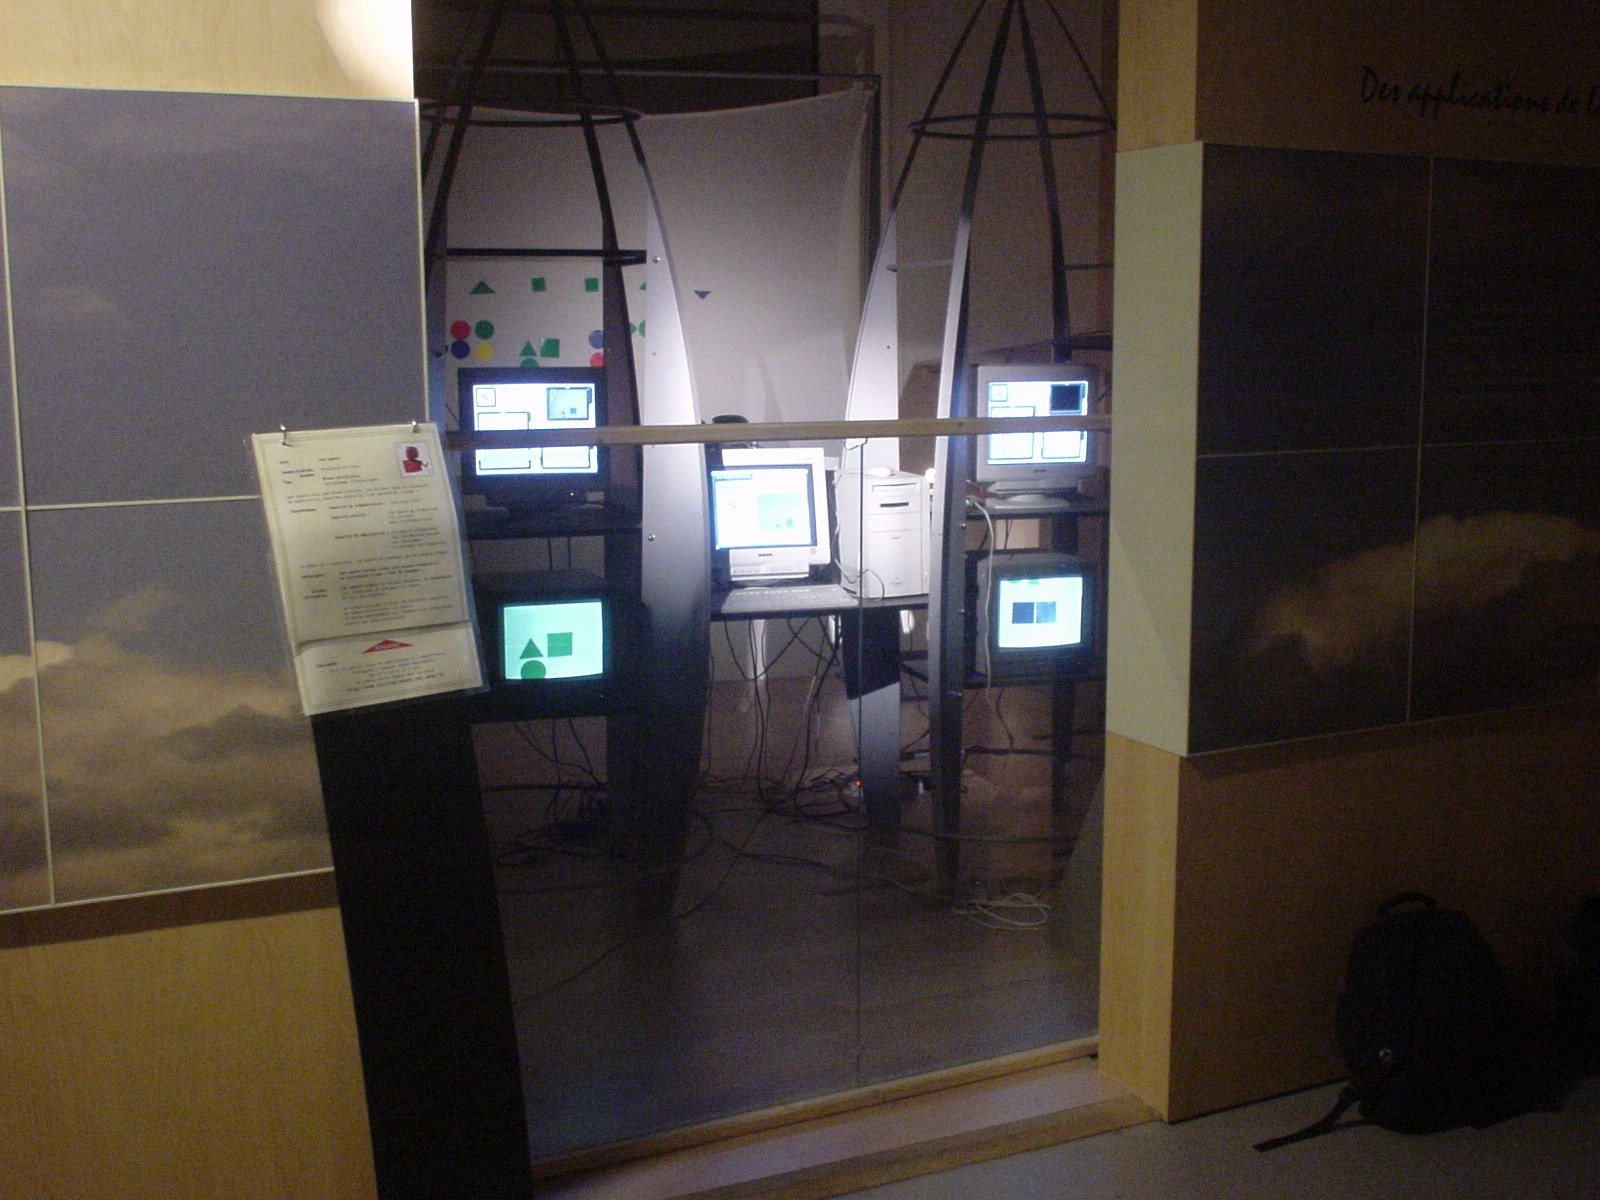
\includegraphics[width=.65\textwidth]{chap9/figs/th4}}
\caption{\label{fig:palais} 
Talking Heads Installation at the Palais de la D\'{e}couverte. It featured new fancy structures that 
made the installation more attractive visually. Daily explanations were given to visitors 
by the staff of the Palais de la D\'{e}couverte.} 
\end{figure}

\section{The Portable Talking Heads} 

As news of the Talking Heads experiment was spreading, more and more inquiries were made to \is{portable Talking Heads}
show the experiment live in other locations. So we made a portable version (see \figref{fig:road}) that could easily 
be installed and assembled. Initially this version was used to link into the live 
teleportation infrastructure, but once the N01SE exhibition was finished, it was used to develop focused 
experiments, in particular on color language. 

\begin{figure}[htbp]
  \centerline{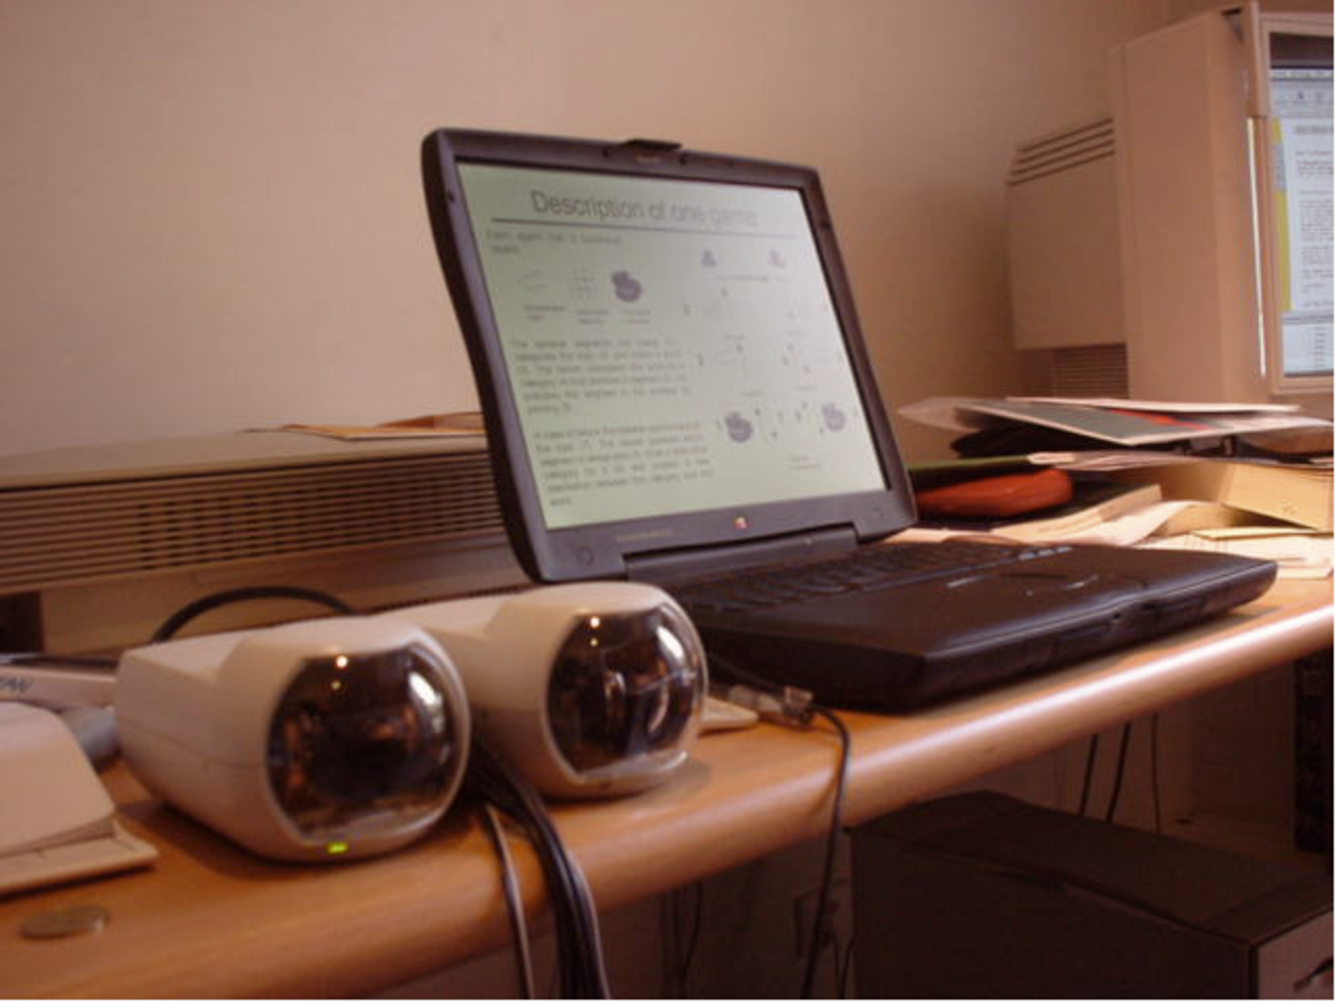
\includegraphics[width=.60\textwidth]{chap9/figs/road}}
\caption{\label{fig:road} 
Portable installation with two pan-tilt cameras and a portable computer that was able to run the TH software.}
\end{figure}

Some of the noteworthy locations where the portable installation was used are the following: 

1. The {\itshape European Conference on Artificial Life} at the EPFL in Lausanne (Switzerland) in september 1999. 
Papers on computational and robotic 
models of language evolution were (and still are) greeted with hostility at linguistics conferences (even 
conferences on computational linguistics) and they are still routinely rejected for linguistics journals, as 
being `irrelevant' for understanding more about human language. 
However the Artificial Life conferences and journals welcomed the approach from the beginning. This is 
not surprising because agent-base modeling is one of the main tools used in that field and an evolutionary 
stance is seen as obvious to biologists. The Lausanne conference was organised in line with earlier 
conferences on artificial life, showing work on life-like robots, computer simulations, and new chemically based 
forms of life. It also featured a series of live demos. The portable demonstration of the Talking Heads was part 
of these demonstrations, set up to accompany a presentation at 
the conference by Luc Steels and Fr\'{e}deric Kaplan\footnote{
The paper published for this conference is \cite{Steels:1999}.}
It was linked in with the ongoing experiment during Laboratorium in Antwerp. 

\begin{figure}[htbp]
  \centerline{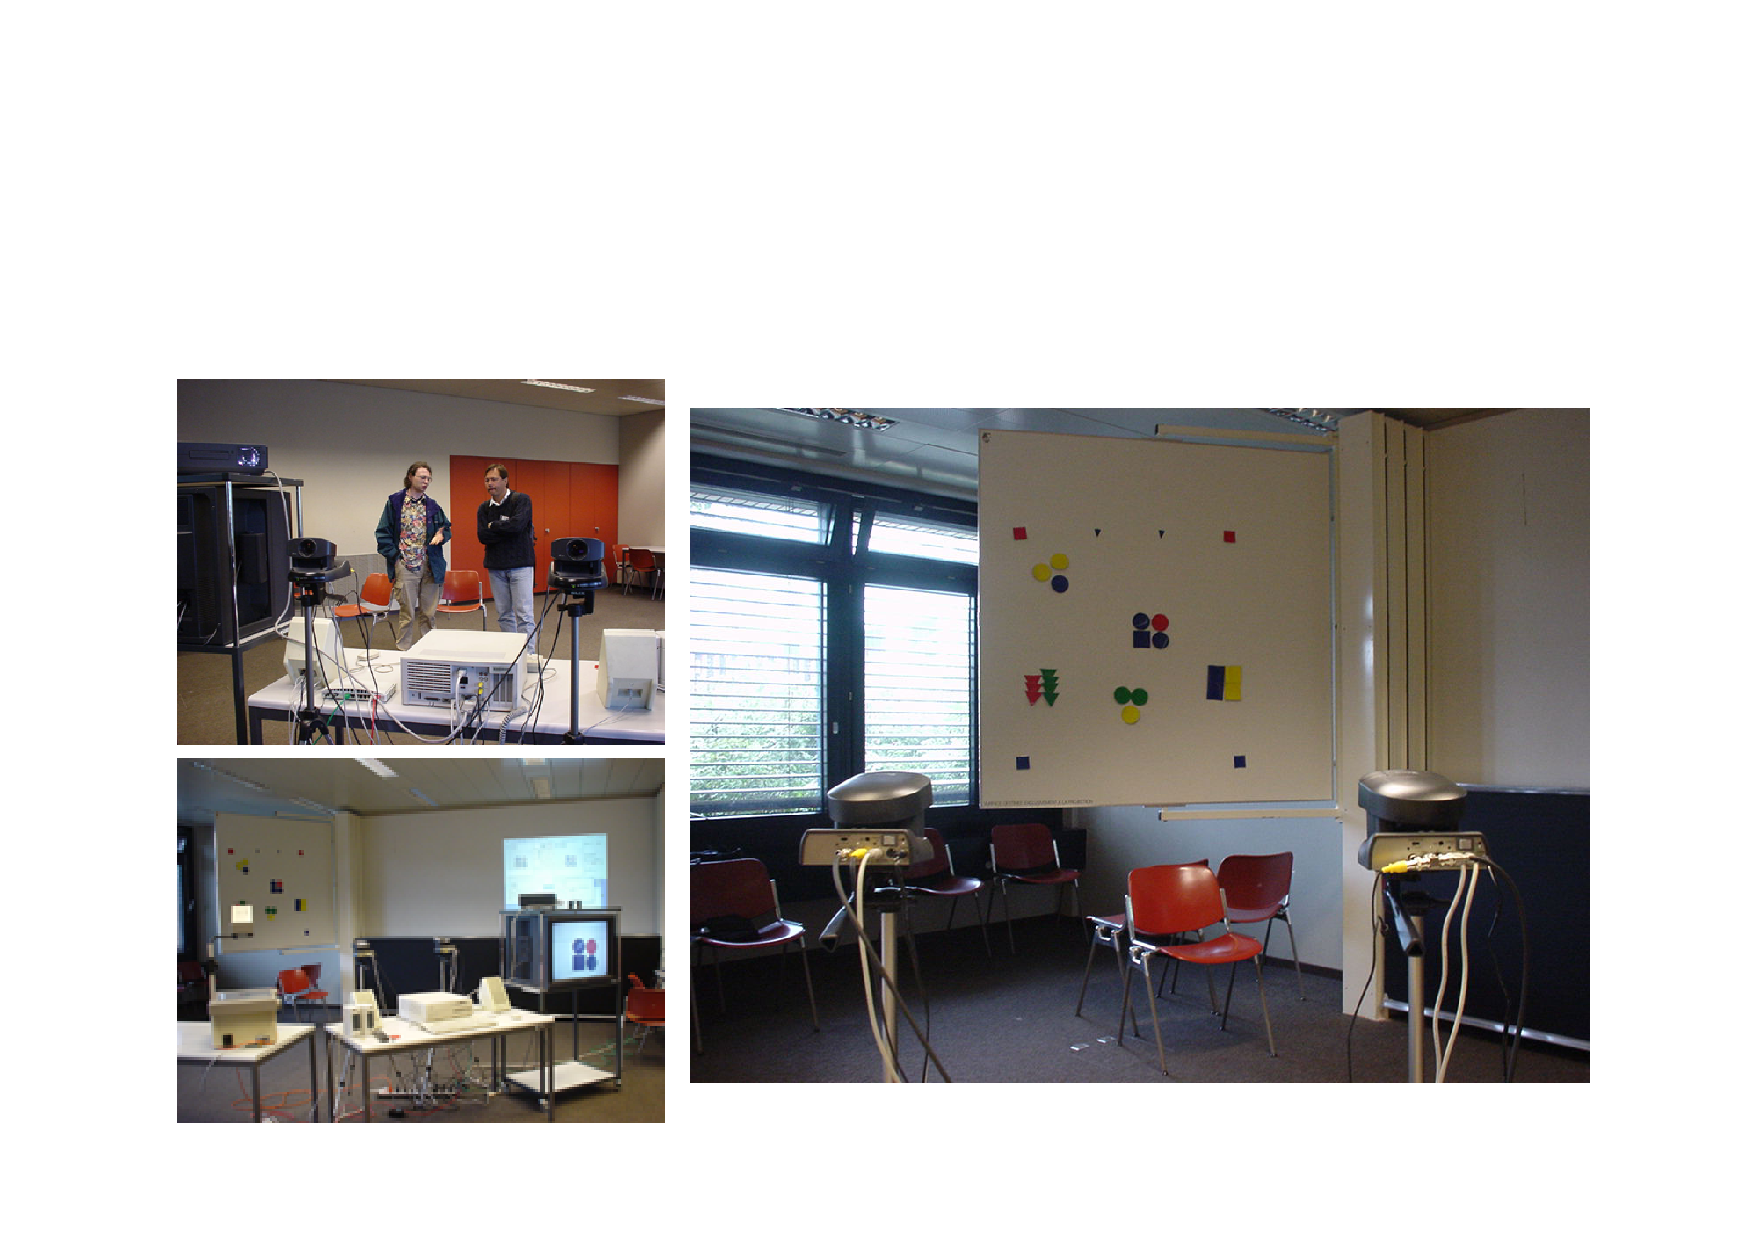
\includegraphics[width=.90\textwidth]{chap9/figs/Lausanne}}
\caption{\label{fig:lausanne} 
Live installation and demonstration of the Talking Heads experiment at the European Conference on Artificial 
Life in 1999.}
\end{figure}

2. The {\itshape Neuer Aachener Kunstverein} in Aachen (Germany) in collaboration with the 
RWTH (the technical university of Aachen) organised a general exhibition on modelling called 
Modell-Modell. Within this framework, artist Anne-Mie van Kerckhoven invited Luc Steels to cooperate in a laboratory on 
language and color called "Cyberlabor - Chromosophy". As part of this laboratory, the portable Talking Heads 
experiment was installed and ran from 5 may to 16 june 2000. It featured not only the portable Talking Heads, 
which was demonstrated live, but also posters, talks about the project and additional art works. 

3. The portable Talking Heads was also featured in an exhibition at the {\itshape Ludo Mich Gallery} in Antwerp. This 
exhibition focused on color again and showed several other pieces related to color and color perception. 
It was accompanied by a very well attended gallery talk. 

\begin{figure}[htbp]
  \centerline{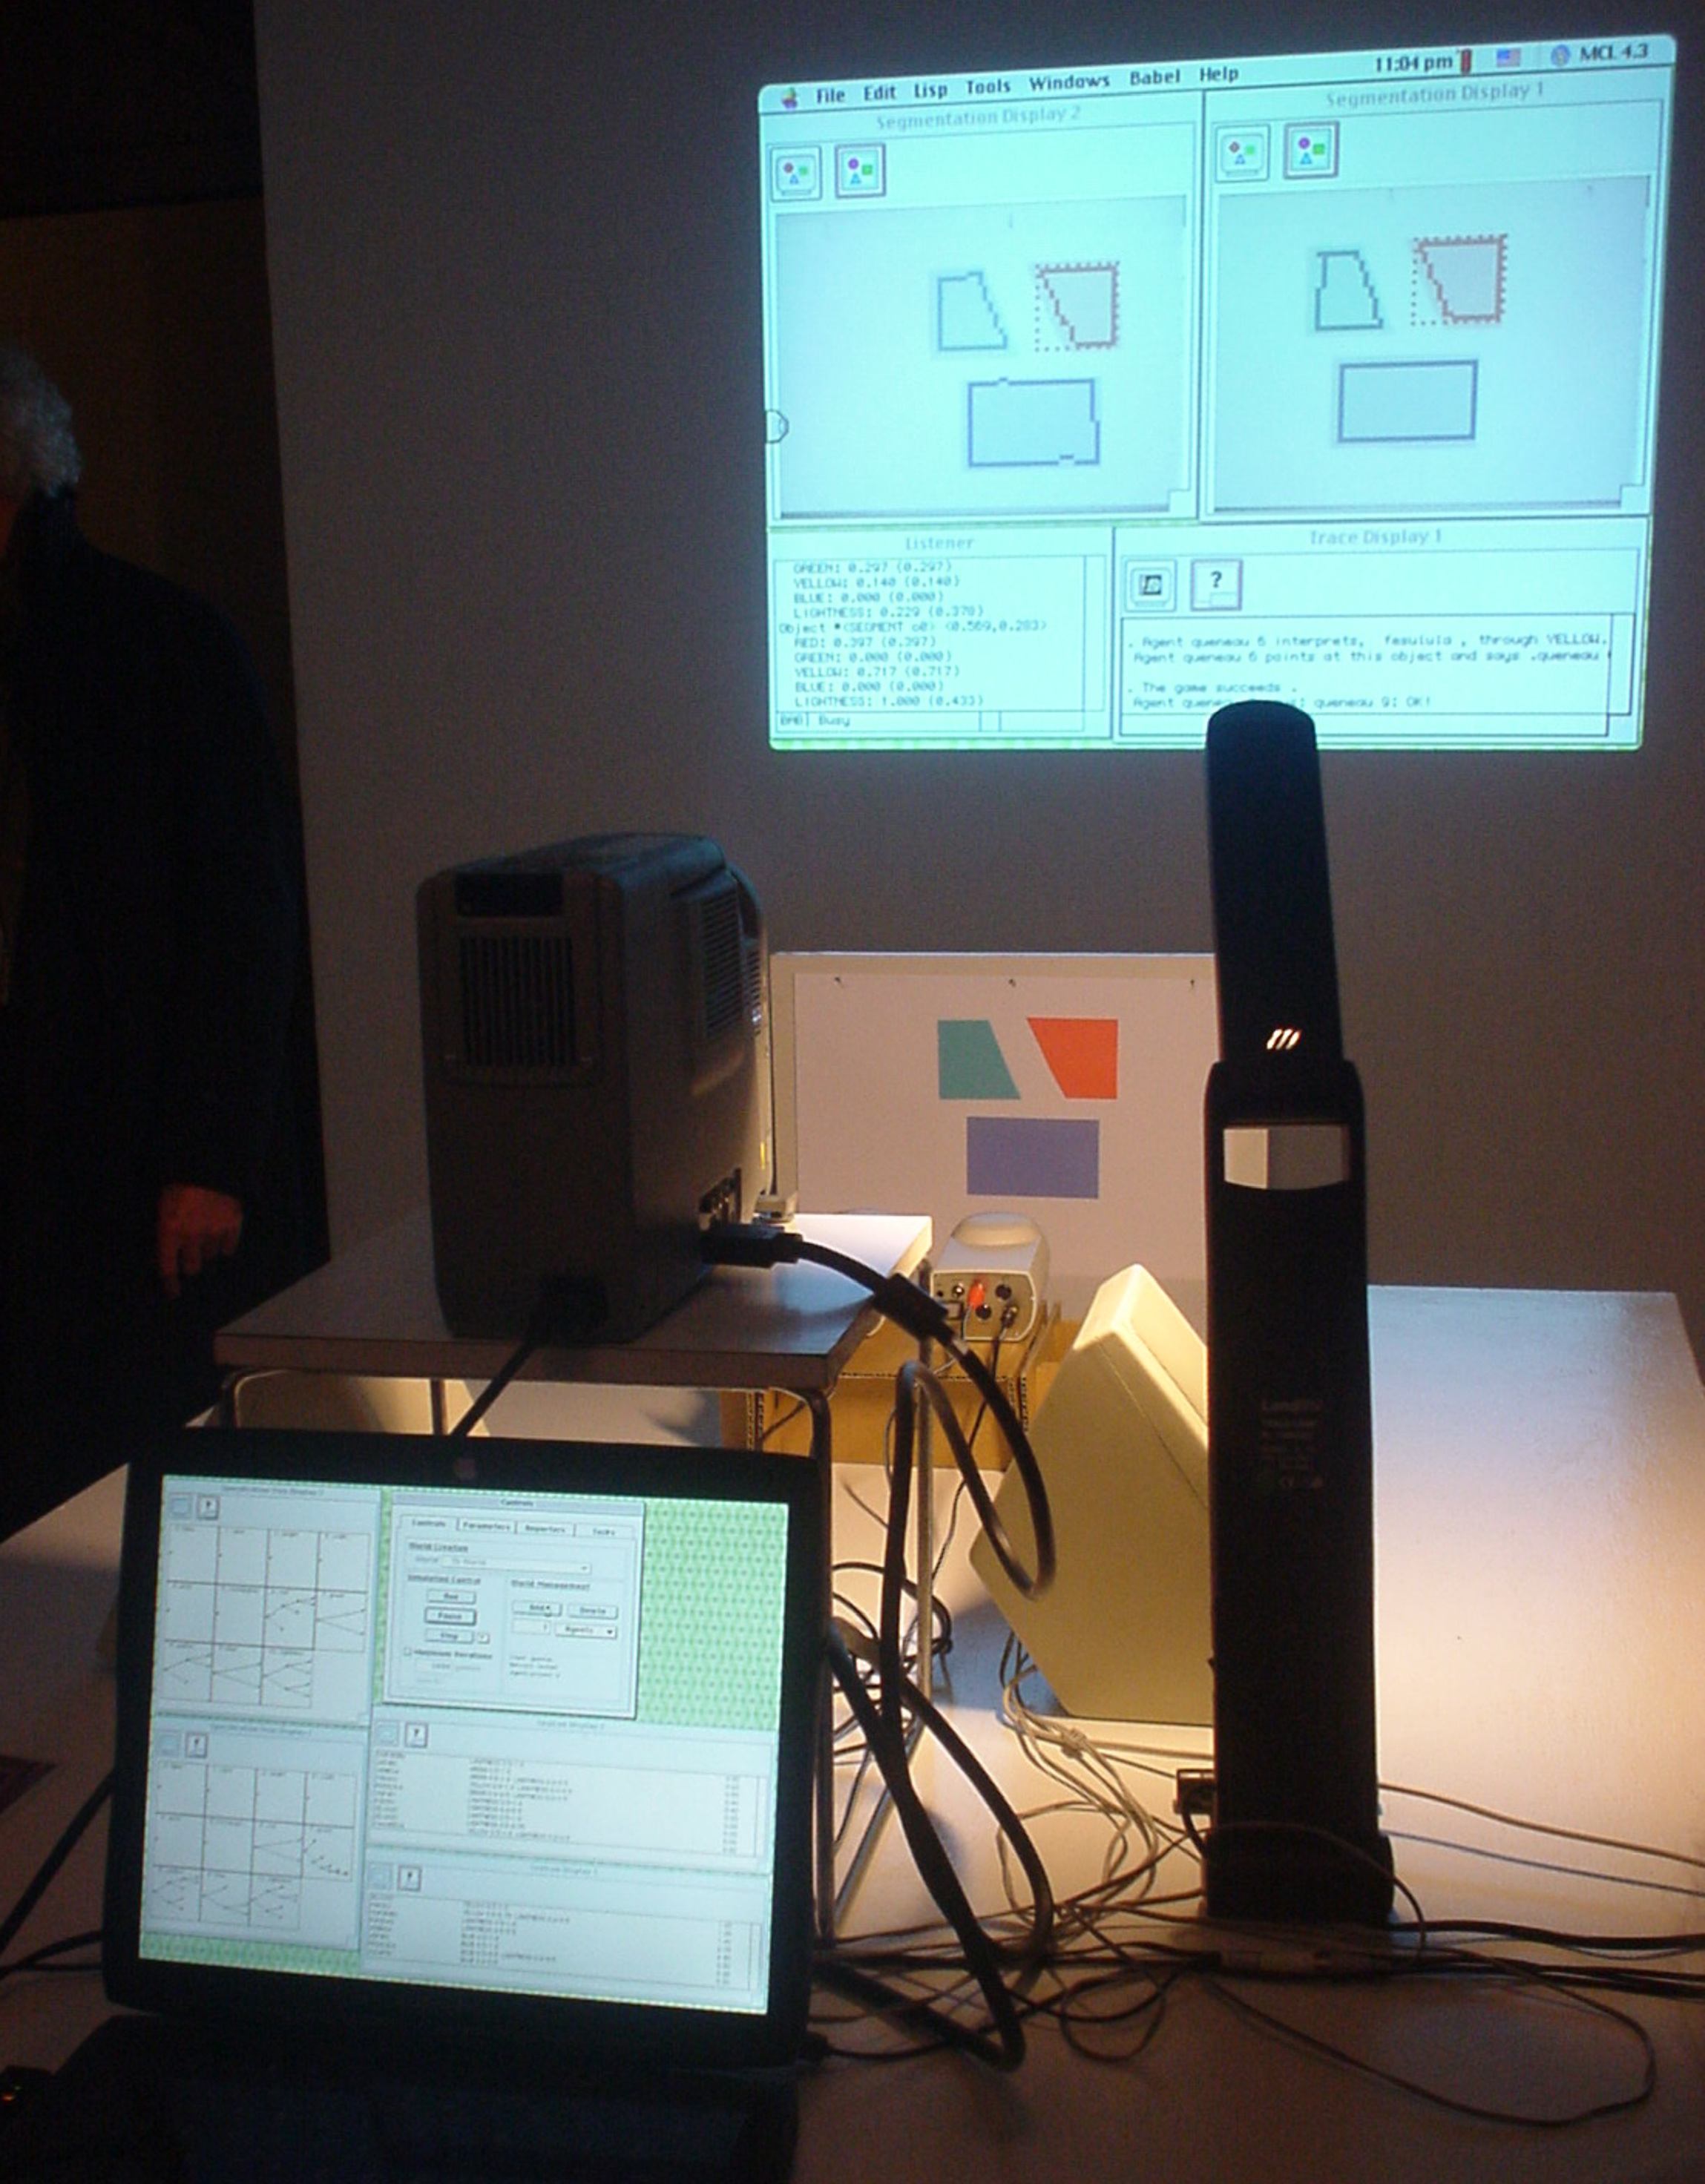
\includegraphics[width=.80\textwidth]{chap9/figs/mich-gallery}}
\caption{\label{fig:mich} 
Live installation at the gallery of Ludo Mich in Antwerp. There was no white board but different 
small pancartes with possible scenes (see in the middle of the picture). The game was displayed much larger against
the back wall.}
\end{figure}

\section{Look into the Box} 

The {\itshape Mus\'ee d'Art Moderne} in Paris organised a solo exhibition of artist Olafur Eliasson entitled 
``Chaque matin je me sens diff\'erent. Chaque soir je me sens le m\^eme" between 
22 march and 12 may 2002.\cite{Scherf:2002} Olafur Eliasson is known for his thorough 
investigations of color, such as using monochromatic light to create an artificial sun in the Modern Tate
Gallery in London (2003). Eliasson invited Luc Steels to jointly work out a new interpretation of the 
Talking Heads Experiment, which became ``Look into the Box". Nicolas Neubauer, a master student working at 
that time at the Sony Computer Science Laboratory, was the chief implementer together with Angus McIntyre.  
The set-up and results are described in detail in \cite{Steels:2004} and \cite{Neubauer:2004}.\is{Museum of Modern Art installation}

``Look into the box" consisted of a box in which a camera was mounted that would take a picture of the 
eye of a person who looked into the box. The eye was then projected much bigger on a wall opposite to the box, 
which in itself gave a very strong visual effect (see \figref{fig:lookintobox}). 
At the same time two artificial agents looked at the 
eye color and played a color language game. Visitors to the exhibition could hear the dialog between the agents 
and follow on a nearby screen the progression in the emergence of a color vocabulary. During the course of the 
exhibition an artificial color language emerged, reflecting the eye and skin color of visitors. 
\begin{figure}[htbp]
  \centerline{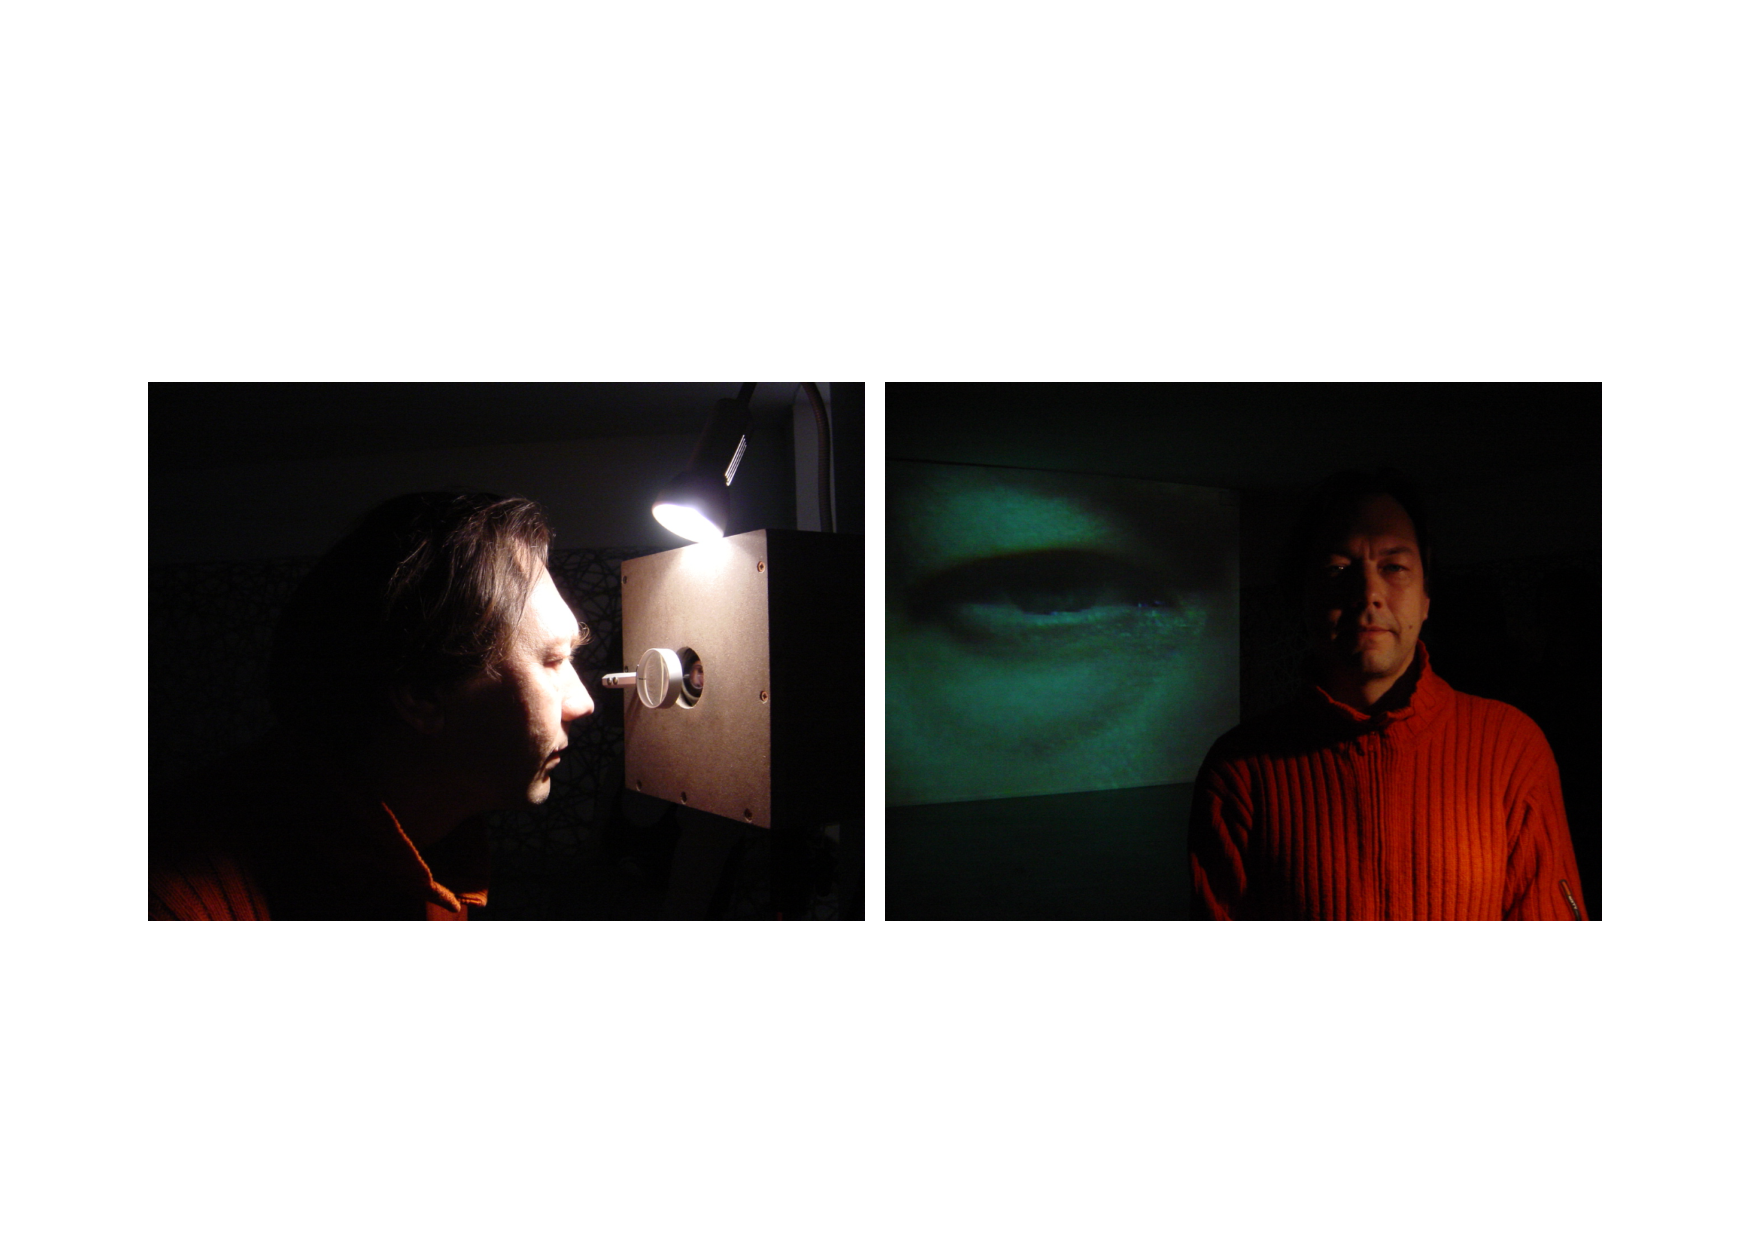
\includegraphics[width=.95\textwidth]{chap9/figs/look-into-box}}
\caption{\label{fig:lookintobox} 
Look into the Box installation at the Paris Museum of Modern Art. Left: Box with camera inside. A lens would make 
the eye look bigger for the camera. Right: Projection of the eye on a big screen.}
\end{figure}

This experiment was fundamentally 
different from the original Talking Heads experiment because it was no longer a discrimination game
but a description game. The agents extracted the main colors from the image of the eye and then described them to 
another agent. Moreover the domain was now restricted to the color domain, which had meanwhile 
become a focal topic of research in the lab.\cite{Steels:2005}

\begin{figure}[htbp]
  \centerline{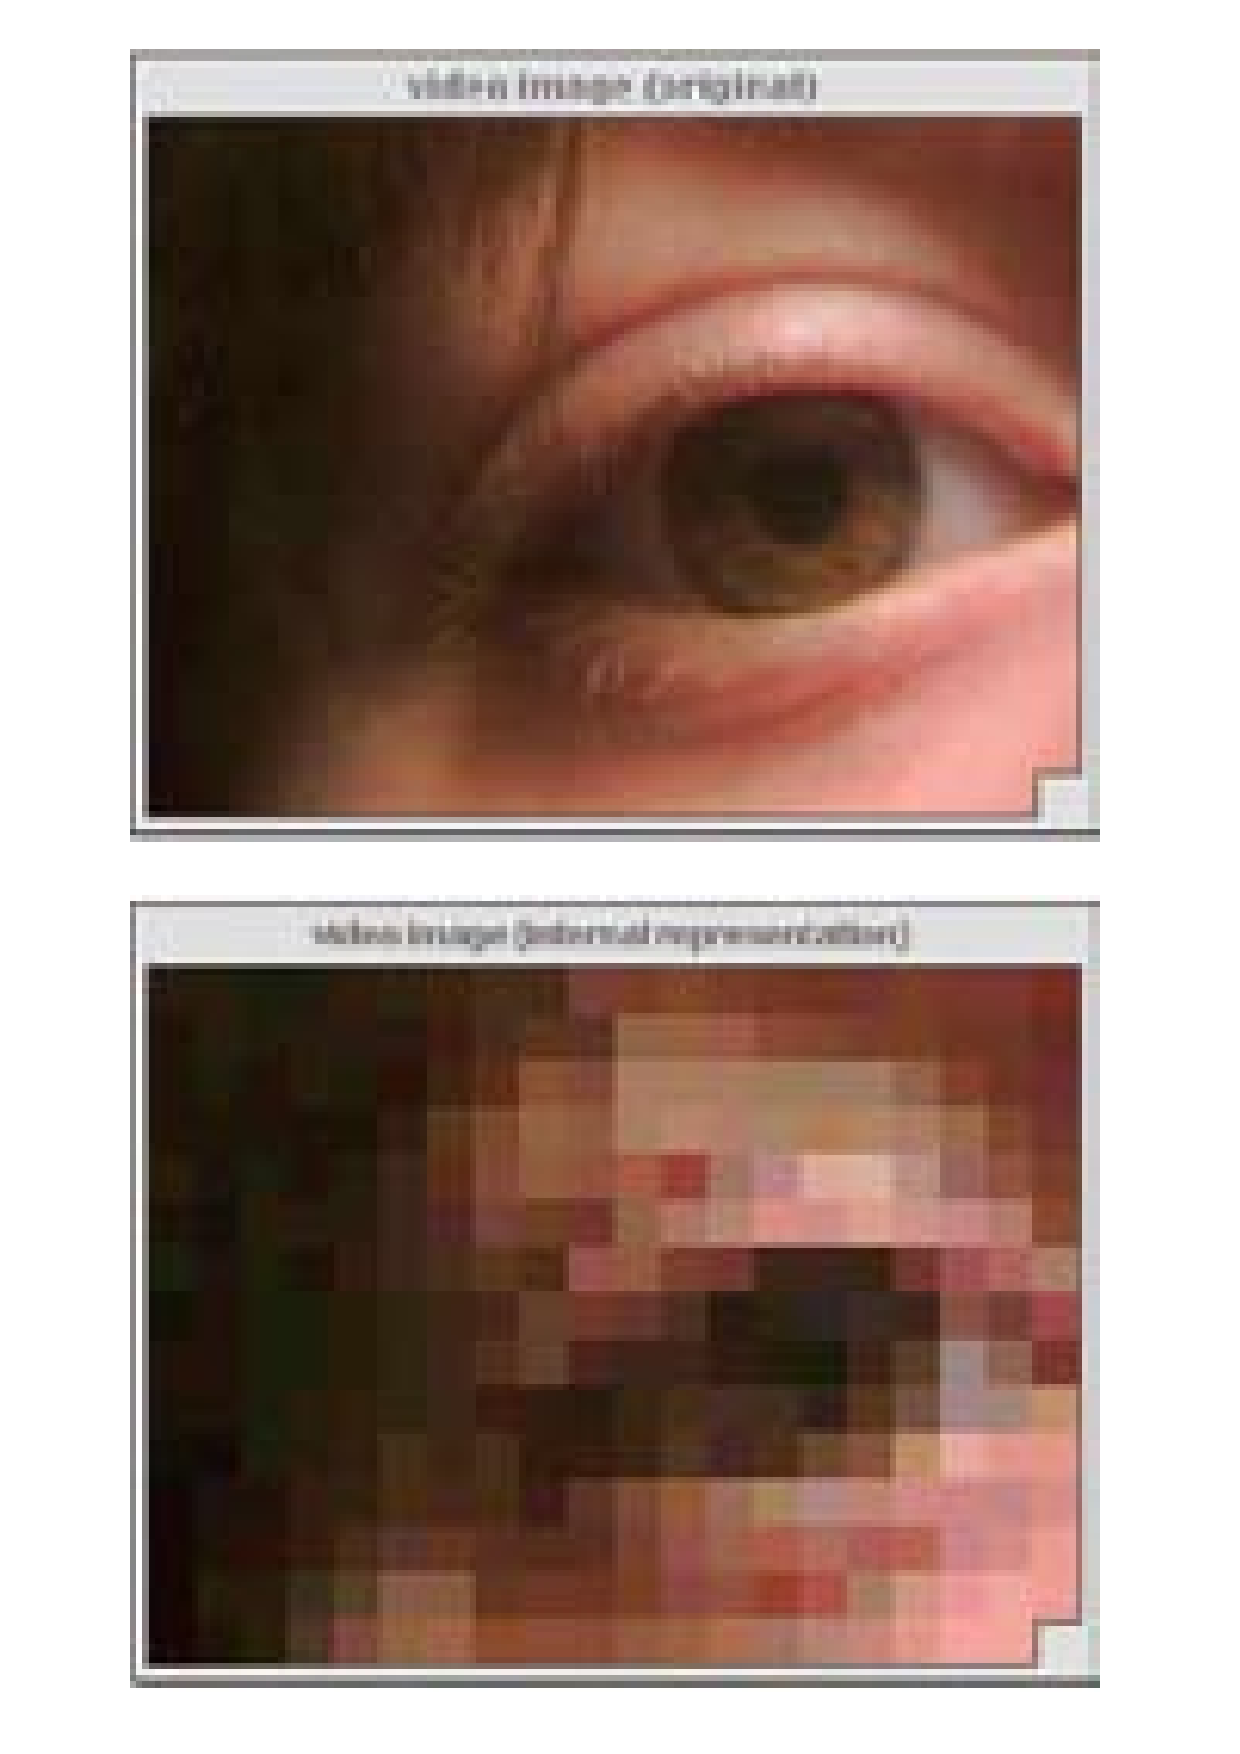
\includegraphics[width=.30\textwidth]{chap9/figs/eyes}
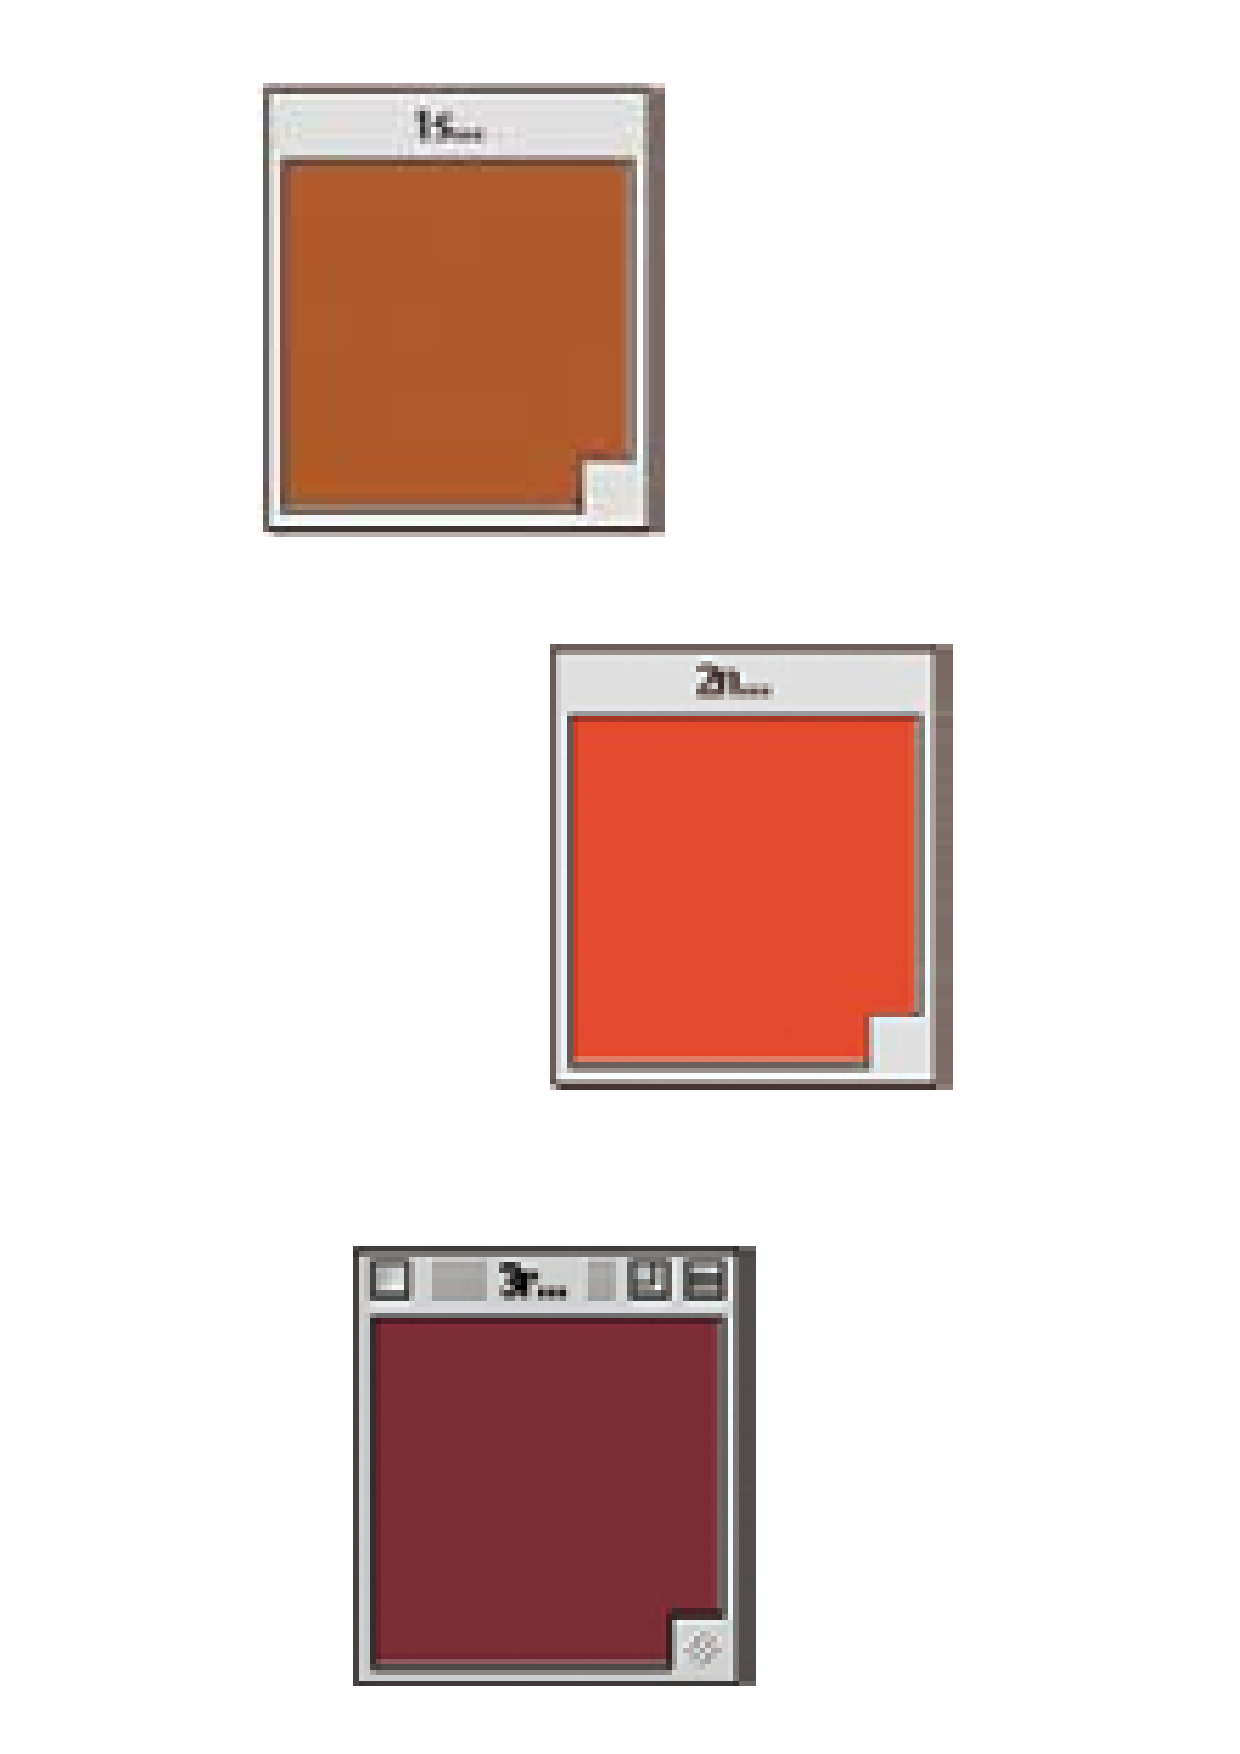
\includegraphics[width=.30\textwidth]{chap9/figs/identified-colors}}
\caption{\label{fig:eyes} 
Example interaction of the "Look into the Box" art piece. 
Left: Top and pixilated eye of a spectator. Right: the main colors that 
were extracted from this image. Agents played language games to describe these eye colors.}
\end{figure}

The 'Look into the Box' installation was shown again at several locations. One was in July 2003  
in the context of a yearly music festival in Spoleto. In 2003, the theme of semiotic dynamics was 
chosen and various presentations and 
discussions were held curated by the Italian semiotician Paolo Fabbri. A new installation of 
Look into the Box was realised and operated (see \figref{fig:spoleto}). A system for playing language games 
with human users, created by Tony Belpaeme of the VUB AI Lab, was also demonstrated. This system was intended
to collect data about color category prototypes and names from human speakers in order to gather more data
about color language in discrimination games. 

\begin{figure}[htbp]
  \centerline{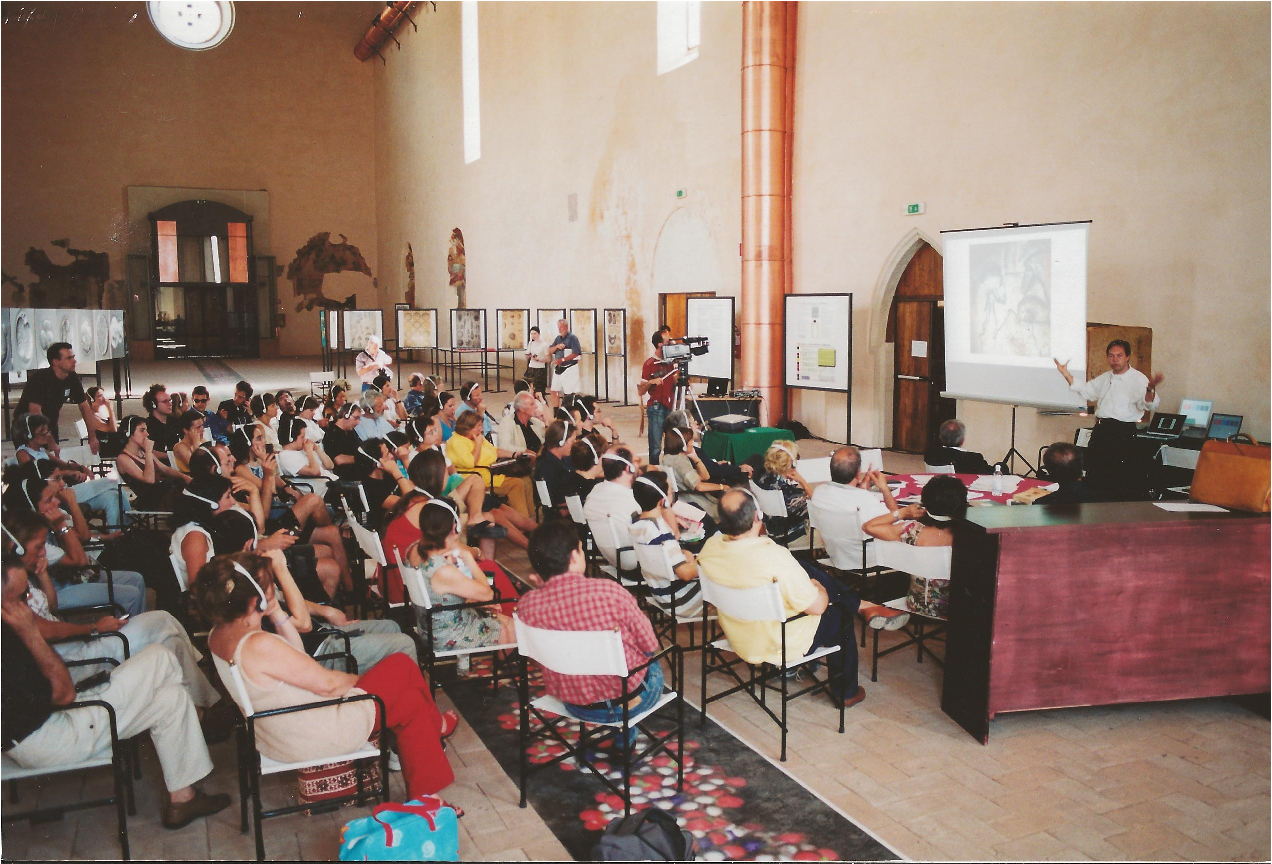
\includegraphics[width=.65\textwidth]{chap9/figs/ital-talk}
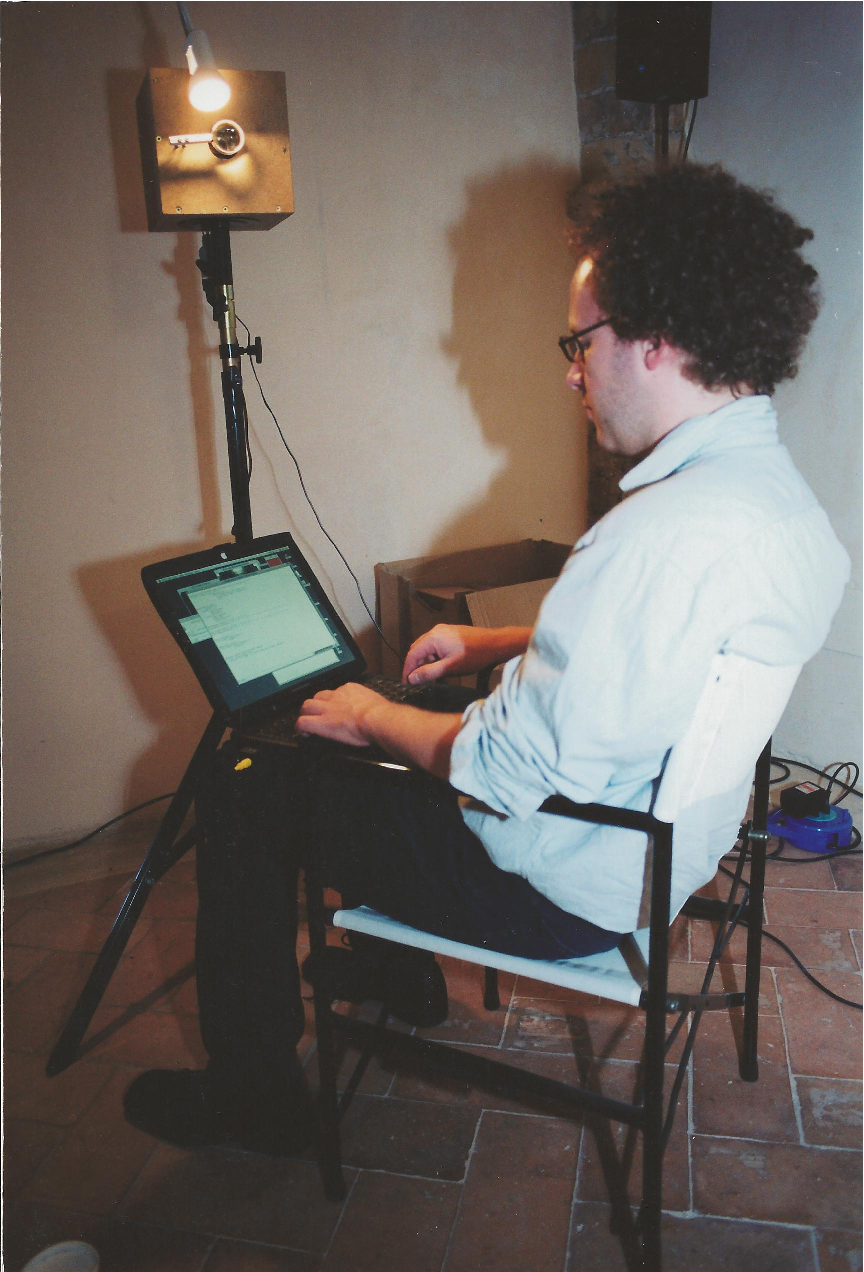
\includegraphics[width=.30\textwidth]{chap9/figs/ital2}}
\caption{\label{fig:spoleto} 
Left: Presentation by Luc Steels at the Spoleto Science Festival. Right: Nicolas Neubauer debugging 
the ``Look into the Box" installation.
 }
\end{figure}

The Look into the Box installation was also shown during the ``Intensive Science" exhibitions organised in october 
2006 on the occasion of the 10th anniversary of the Sony Computer Science Laboratory.\is{Intensive Science exhibition}
It was first shown in Paris at 
the exhibition space ``La Maison Rouge" near the Bastille in Paris, which featured science/art installations 
and collaborations involving members of the Sony Computer Science Laboratory, including work by Atau Tanaka, 
Francois Pachet in collaboration with Jazz pianist Albert van Veendaal, Peter Hanappe in collaboration with 
photographer Armin Linke, Frederic Kaplan in collaboration with the design school of EPFL in Lausanne. 
The same exhibition traveled to Tokyo where it was shown in the Sony Explorascience museum from 22 december 2006 
to 12 february 2007 (see \figref{fig:intensive-science}). 
\begin{figure}[htbp]
  \centerline{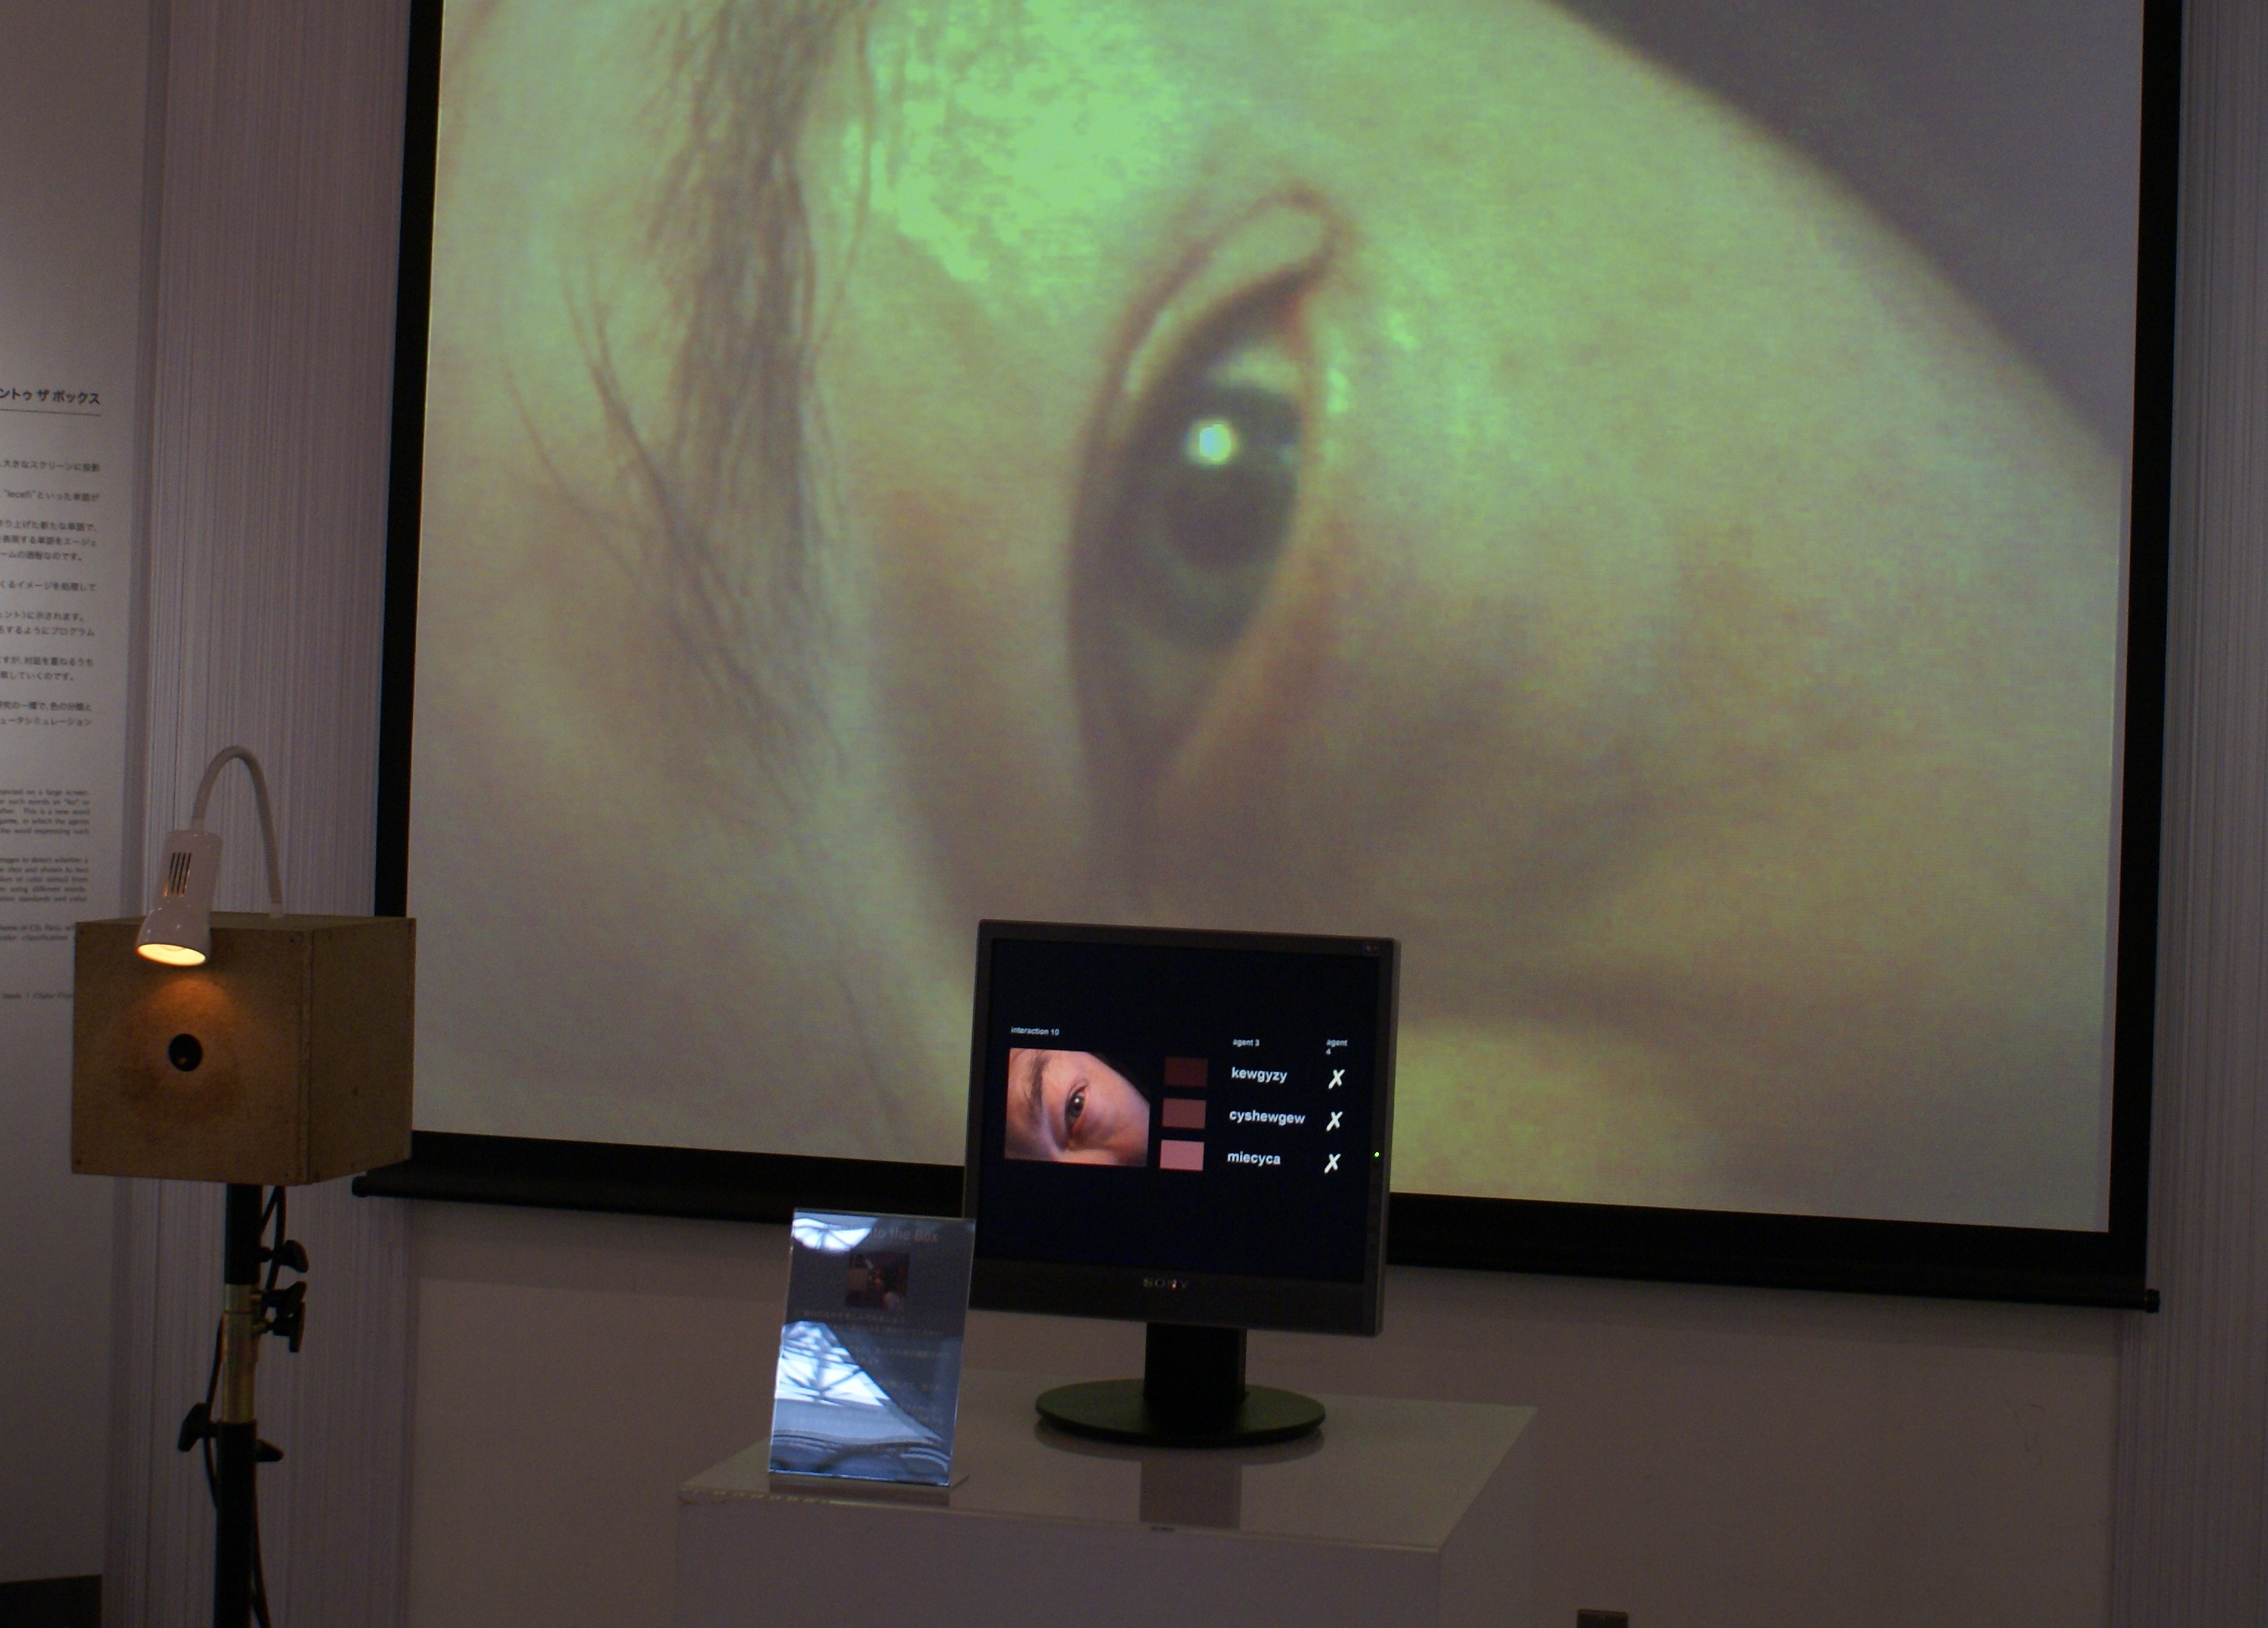
\includegraphics[width=.80\textwidth]{chap9/figs/explorascience}}
\caption{\label{fig:intensive-science} 
Installation at the Tokyo Explorascience Museum. The box is in the left corner. The eye is projected on a 
big screen. A smaller screen shows the image captured by the camera, the colors recognised, and the words used by 
the agents.}
\end{figure}
\section{Conclusions}

The many installations and experiments taught us a lot about how it was possible to technically set up 
and maintain a distributed network of agents grounding their activities in the real world through cameras. 
These pioneering experiments happened at a time when the Internet was not as common as today and not as stable. 
It was before up- and down-loading and 'apps' became widespread and sufficient bandwidth was available 
even in private homes. The experiments were stopped around 2002 because
they took a lot of time and not much more could be learned from a technical and scientific point of view. 

The installations were also one of the pioneering attempts to develop a strong interaction between art and science, 
which today are more common and more recognised than they were in the late nineties.
They were conceived to be part of exhibitions and well established artists, such as Olafur Eliasson, took great 
interest and collaborated to give them a twist to function better within an art context. 
The context of an exhibition is a very effective way to reach an audience
that has normally no access to ongoing scientific experiments. It also generated a stream of newspaper articles, 
and contributions to radio and television programs, which normally pay only little attention to what goes in science. 

The experiments also taught us a lot about the interaction between humans and artificial agents. The idea that 
a benign symbiosis between artificial agents and humans was possible proved to be naive. There are too many 
people around with sufficient computer 
skill but without any ethical consciousness. They see no problem in destroying computational infrastructure simply for 
their own joy. More recent examples show that these hackers go much further, using their power to do harm or widespread
theft. As artificial systems will never be immune to this behavior, it is probably not possible to imagine a future in which 
there are autonomous robotic agents, not because the robots would be harmful in themselves but because of 
the use some individuals will most likely make of them. 

Finally, the experiments taught us that the proposed mechanisms for lexicon and concept formation and for reaching 
coherence worked out. The lateral inhibition learning dynamics and the structural coupling 
between lexicon formation and concept formation used by the agents proved later not only relevant for 
lexicon formation but also for grammar. On the other hand this dynamics is not robust enough in the face 
of extreme uncertainty coming from embodiment (i.c. camera disalignment), high population flux, uncertain 
environmental conditions or destructive human user 
interventions. Presumably in such conditions child language and concept learning would also be heavily 
compromised and perhaps impossible. Anthropologists have argued that the origins of language required a strong  
form of sociality which is not found in other primate species.\cite{Knight:2014}. 
The experiment indeed confirms that without empathy, respect and a common purpose, a shared language will not come off the ground. 

